\documentclass[landscape,a0paper,fontscale=0.45,margin=1.5cm]{baposter}
%\documentclass[landscape,paperwidth=1682mm,paperheight=1189mm,fontscale=0.4,margin=3cm]{baposter}

\usepackage{calc}
\usepackage{graphicx}
\usepackage{amsmath}
\usepackage{amssymb}
\usepackage{relsize}
\usepackage{multirow}
\usepackage{rotating}
\usepackage{bm}
\usepackage{enumitem}
\usepackage{booktabs}
\usepackage{relsize}		% For \smaller
\usepackage{url}			% For \url

\usepackage{graphicx}
\usepackage{multicol}
\usepackage{subcaption}
\captionsetup{compatibility=false}

\usepackage{nameref}
%\usepackage{times}
%\usepackage{helvet}
%\usepackage{bookman}
\usepackage{palatino}
%% Pablo's personal packages
%% AMS unofficial LateX proceeding template:
%%    http://www.cimms.ou.edu/~lakshman/ametsoc/
%%\usepackage[hypertex]{hyperref}
%% end personal packages

%\newcommand{\captionfont}{\footnotesize}

\graphicspath{{images/}{./images}}
\usetikzlibrary{calc}


\newcommand{\Matrix}[1]{\begin{bmatrix} #1 \end{bmatrix}}
\newcommand{\Vector}[1]{\begin{pmatrix} #1 \end{pmatrix}}

\newcommand*{\norm}[1]{\mathopen\| #1 \mathclose\|}% use instead of $\|x\|$
\newcommand*{\abs}[1]{\mathopen| #1 \mathclose|}% use instead of $\|x\|$
\newcommand*{\normLR}[1]{\left\| #1 \right\|}% use instead of $\|x\|$

\newcommand*{\SET}[1]  {\ensuremath{\mathcal{#1}}}
\newcommand*{\FUN}[1]  {\ensuremath{\mathcal{#1}}}
\newcommand*{\MAT}[1]  {\ensuremath{\boldsymbol{#1}}}
\newcommand*{\VEC}[1]  {\ensuremath{\boldsymbol{#1}}}
\newcommand*{\CONST}[1]{\ensuremath{\mathit{#1}}}

\DeclareMathOperator*{\argmax}{arg\,max}
\DeclareMathOperator*{\diag}{diag}
\DeclareMathOperator*{\argmin}{arg\,min}
\DeclareMathOperator*{\vectorize}{vec}
\DeclareMathOperator*{\reshape}{reshape}

%\font\dsfnt=dsrom12

\newcommand{\SNN}{\ensuremath{\mathbb N}}
\newcommand{\SRR}{\ensuremath{\mathbb R}}
\newcommand{\SZZ}{\ensuremath{\mathbb Z}}
%-----------------------------------------------------------------------------
% Matrices of the shape model
\renewcommand{\a}{\VEC\alpha}
\renewcommand{\v}{\VEC v}
\renewcommand{\l}{\VEC l}
\newcommand*{\m}{\VEC{\mu}}
\newcommand*{\M}{\MAT{M}}
\renewcommand*{\P}{\MAT{\Pi}}

%\newcommand{\J}{\SET J}
\newcommand{\J}{\SET{P}}
\newcommand{\Active}{\mathcal{A}}
\newcommand{\Selection}{\mathbf{S}}
\newcommand{\AllSelections}{\mathfrak{S}}
\newcommand{\Params}{\VEC\Theta}

%%%%%%%%%%%%%%%%%%%%%%%%%%%%%%%%%%%%%%%%%%%%%%%%%%%%%%%%%%%%%%%%%%%%%%%%%%%%%%%%
%%%% Some math symbols used in the text
%%%%%%%%%%%%%%%%%%%%%%%%%%%%%%%%%%%%%%%%%%%%%%%%%%%%%%%%%%%%%%%%%%%%%%%%%%%%%%%%

%%%%%%%%%%%%%%%%%%%%%%%%%%%%%%%%%%%%%%%%%%%%%%%%%%%%%%%%%%%%%%%%%%%%%%%%%%%%%%%%
% Multicol Settings
%%%%%%%%%%%%%%%%%%%%%%%%%%%%%%%%%%%%%%%%%%%%%%%%%%%%%%%%%%%%%%%%%%%%%%%%%%%%%%%%
\setlength{\columnsep}{1.5em}
\setlength{\columnseprule}{0mm}

%%%%%%%%%%%%%%%%%%%%%%%%%%%%%%%%%%%%%%%%%%%%%%%%%%%%%%%%%%%%%%%%%%%%%%%%%%%%%%%%
% Save space in lists. Use this after the opening of the list
%%%%%%%%%%%%%%%%%%%%%%%%%%%%%%%%%%%%%%%%%%%%%%%%%%%%%%%%%%%%%%%%%%%%%%%%%%%%%%%%
\newcommand{\compresslist}{%
\setlength{\itemsep}{1pt}%
\setlength{\parskip}{0pt}%
\setlength{\parsep}{0pt}%
}

%%%%%%%%%%%%%%%%%%%%%%%%%%%%%%%%%%%%%%%%%%%%%%%%%%%%%%%%%%%%%%%%%%%%%%%%%%%%%%
%%% Begin of Document
%%%%%%%%%%%%%%%%%%%%%%%%%%%%%%%%%%%%%%%%%%%%%%%%%%%%%%%%%%%%%%%%%%%%%%%%%%%%%%

\begin{document}

%%%%%%%%%%%%%%%%%%%%%%%%%%%%%%%%%%%%%%%%%%%%%%%%%%%%%%%%%%%%%%%%%%%%%%%%%%%%%%
%%% Here starts the poster
%%%---------------------------------------------------------------------------
%%% Format it to your taste with the options
%%%%%%%%%%%%%%%%%%%%%%%%%%%%%%%%%%%%%%%%%%%%%%%%%%%%%%%%%%%%%%%%%%%%%%%%%%%%%%
% Define some colors

\definecolor{silver}{cmyk}{0,0,0,0.3}
\definecolor{yellow}{cmyk}{0,0,0.9,0.0}
\definecolor{reddishyellow}{cmyk}{0,0.22,1.0,0.0}
\definecolor{black}{cmyk}{0,0,0.0,1.0}
\definecolor{white}{rgb}{1,1,1}
\definecolor{red}{rgb}{.9,0,0}
\definecolor{green}{rgb}{0,.3,0}
\definecolor{blue}{rgb}{.11,.14,.96}

\definecolor{darkBlue}{rgb}{.15,0.2, 0.9513}
\definecolor{darkYellow}{cmyk}{0,0,1.0,0.5}
\definecolor{darkSilver}{cmyk}{0,0,0,0.1}

\definecolor{middlegray}{rgb}{.4,.4,.4}
\definecolor{lightgray}{rgb}{.7,.7,.7}

\definecolor{lightgreen}{rgb}{.7,7,.35}
\definecolor{lightlila}{rgb}{.6,.6,.8}
\definecolor{lightorange}{rgb}{.88,.74,.15}
\definecolor{lighterorange}{rgb}{.98,.84,.45}
\definecolor{middleblue}{rgb}{.447,.537,.9513}
\definecolor{lightblue}{rgb}{.447,.537,.6313}
\definecolor{lighterblue}{rgb}{.568,.639,.709}
\definecolor{lighteryellow}{cmyk}{0,0,0.1,0.0}
\definecolor{lightestblue}{rgb}{.6,.7,.8}

%%% Setting Background Image %%%%%%%%%%%%%%%%%%%%%%%%%%%%%%%%%%%%%%%%%%%%%%%%%%
\background{
	\begin{tikzpicture}[remember picture,overlay]%
	\draw (current page.north west)+(-0em,0em) node[anchor=north west]
	{\includegraphics[height=1.01\textheight]{uni_leipzig-bg.jpg}};%{BG_ADMIRARI.jpg}};%
	\end{tikzpicture}
}


%\hyphenation{resolution occlusions}
%%
\begin{poster}%
  % Poster Options
  {
  % Show grid to help with alignment
  grid=false, %true,
  % Number of columns
  columns=4,
  % Column spacing
  colspacing=1.0em,
  % Color style
  bgColorOne= white, %white, %lightgreen, %silver,
  bgColorTwo= lightblue, %white, %middlegray, %lightestblue, %white,
  borderColor=darkBlue, %reddishyellow, %lightorange,
  headerColorOne=lightblue, %darkSilver, %, %lightblue,   %lightblue,
  headerColorTwo=lighterblue, %lightgray, 
  headerFontColor=black, %lightorange, %black,
  boxColorOne=blue, %darkSilver, %darkSilver, % %darkYellow,
  boxColorTwo=middleblue, %red, %white,
  % Format of textbox
  textborder=faded,
  % Format of text header
  eyecatcher=true,
  headerborder=open, %none, %open, %none,
  headerheight=0.18\textheight,
  %textfont=\sc, %An example of changing the text font
  headershape=rounded, %smallrounded,
  headershade=shadeLR,
  headerfont=\LARGE\bf,  %%\Large\bf\textsc, %Sans Serif
  textfont={\color{black}\setlength{\parindent}{1.5em}},
  boxshade=shadeLR, %none, %shadeTB, %
  background=shadeTB, %user, %
  linewidth=2.5pt
  }
  % Eye Catcher
  {
  	\begin{tabular}{c}
  	%\vspace{+20em}\\
      \includegraphics[height=8.5em]{IAP-Logo-DE_Blau_RGB.png}\\
      \vspace{+1.5em}
      \hspace{-2em}
\includegraphics[height=9.9em]{Leibniz-Gemeinschaft-Logo-D_schwarz-300dpi.jpg}
\end{tabular}
      %\includegraphics[height=6.0em]{logo_small-ac3.png}
      %\hspace{3em}
      %\includegraphics[height=3.0em]{PosterNumber.png}
  }
  % Title
  {
  	Characterization of Arctic aerosol and optically-thin clouds from the
  	middle troposphere\\ to the lower stratosphere by means of lidar
  	backscatter and depolarization ratio
  }
  % Authors
  {\vspace{+1.2em} \textbf{Pablo Saavedra~Garfias}$^{1}$ (Contact: \url{garfias@iap-kborn.de}), 
  	Anne-Claire Billault-Roux$^{2}$, Josef Höffner$^{1}$, Jan Froh$^{1}$, Frederik Ernst$^{1}$,
  	Gerd Baumgarten$^{1}$,\\ Alsu Mauer$^{1}$, Thorben Lüke-Mense$^{1}$, Rolf Rüfenacht$^{2}$, Michael Strotkamp$^{3}$,
  	Martin Flügge$^{4}$\\
  	\vspace{+1em}
    $^1$Leibniz Institute of Atmospheric Physics, Kühlungsborn, Germany\\
    %$^2$University of Cologne, Institute of Geophysics and Meteorology\\
    $^2$Federal Office of Meteorology and Climatology MeteoSwiss, Payerne Switzerland\\
    $^3$Fraunhofer-Institut für Laserphysik, Aachen, Germany\\
    $^4$Andøya Space, Andenes, Norway
    %% {\color{blue} \url{www2.meteo.uni-bonn.de/admirari}}
   }
  % University logo
  {% The makebox allows the title to flow into the logo, this is a hack
   % because of the L shaped logo.
    %\begin{tabular}{r}
   	%\vspace{+20em}\\
    
\includegraphics[height=8em]{egu26-blue-circle-logo.png}
    %\end{tabular}   
  }

%%%%%%%%%%%%%%%%%%%%%%%%%%%%%%%%%%%%%%%%%%%%%%%%%%%%%%%%%%%%%%%%%%%%%%%%%%%%%%
%%% Now define the boxes that make up the poster
%%%---------------------------------------------------------------------------
%%% Each box has a name and can be placed absolutely or relatively.
%%% The only inconvenience is that you can only specify a relative position 
%%% towards an already declared box. So if you have a box attached to the 
%%% bottom, one to the top and a third one which should be in between, you 
%%% have to specify the top and bottom boxes before you specify the middle 
%%% box.
%%%%%%%%%%%%%%%%%%%%%%%%%%%%%%%%%%%%%%%%%%%%%%%%%%%%%%%%%%%%%%%%%%%%%%%%%%%%%%
    %
    % A coloured circle useful as a bullet with an adjustably strong filling
    \newcommand{\colouredcircle}{%
      \vspace{1em}\tikz{\useasboundingbox (-0.2em,-0.32em) rectangle(0.2em,0.32em); \draw[draw=black,fill=lightblue,line width=0.03em] (0,0) circle(0.28em);}\hspace{0.8em}}

% PSG: my ancillary commands:
\newcommand{\polarstern}{{EULIAA-IR1}\,}
\newcommand{\euliaa}{{EULIAA-IR1}\,}
\newcommand{\mosaic}{\emph{MOSAiC}\,}
\newcommand{\refp}[1]{[\ref{#1}]}
% ----/

%%%%%%%%%%%%%%%%%%%%%%%%%%%%%%%%%%%%%%%%%%%%%%%%%%%%%%%%%%%%%%%%%%%%%%%%%%%%%%
  \headerbox{1.- Research Objectives}{name=objective,column=0,span=1,row=0}{
%%%%%%%%%%%%%%%%%%%%%%%%%%%%%%%%%%%%%%%%%%%%%%%%%%%%%%%%%%%%%%%%%%%%%%%%%%%%%%
Aerosols and high altitude clouds in the Arctic have an important role in the radiative energy budget by influencing the net gain or loss of radiative heat. Aerosols are the main nucleation source for the formation of high altitude clouds and responsible to alter cloud properties.

\begin{tabular*}{0.95\textwidth}[h!]{lr}
	\begin{minipage}{0.7\textwidth}
		\vspace{-4em}
		 Ground-based lidars are well-suited to observe aerosol and optically-thin clouds, however, in remote locations with challenging environments lidars are scarce.
		 To overcome this limitation, a compact mobile Rayleigh-Mie-Resonance lidar has been recently developed as part of the European Lidar Array for Atmospheric Climate Monitoring (EULIAA) {\url{https://euliaa.eu}}.
	%{\small Of main interest is the wintertime/early spring legs 1 to 3 of the \mosaic expedition
		%~\refp{bib:Shupe2022} when 
	%	sea ice leads occured. Instrumention and data set are mainly provided by the Atmospheric Radiation Measurement’s (ARM) Mobile Facility 1 (AMF-1) and by the OCEANET-Atmosphere container from TROPOS.}
	\end{minipage}
	&
	\hfill
\includegraphics[scale=0.33]{cropped-Logo-Euliaa.png}	
\end{tabular*}
\\
The first EULIAA system is a high resolution Doppler infrared (770~nm wavelength) mobile, compact (1 m$^3$) autonomous lidar (\euliaa). The \euliaa senses the atmosphere up to the mesosphere with three field-of-view (FOV): Zenith, 30$^\circ$ off-zenith North-South and East-West. Doppler spectral measurements allow the retrieval profiles of the wind, particle (Mie scattering $\beta_p$) and molecular (Rayleigh scattering $\beta_m$) backscatter coefficient, and depolarization ratio ($\delta_\circ$) for zenith observations.

This contribution focus on \euliaa capabilities to characterize:
\begin{itemize}
	\item tropospheric aerosols and thin-clouds,
	\item stratospheric aerosols and polar stratospheric clouds.
\end{itemize}
 %\vspace{-4.5em}

}
%%%%%%%%%%%%%%%%%%%%%%%%%%%%%%%%%%%%%%%%%%%%%%%%%%%%%%%%%%%%%%%%%%%%%%%%%%%%%%
\headerbox{2.- Arctic Observations by EULIAA-IR}{name=andoya,column=0,span=1,below=objective}{
%%%%%%%%%%%%%%%%%%%%%%%%%%%%%%%%%%%%%%%%%%%%%%%%%%%%%%%%%%%%%%%%%%%%%%%%%%%%%%
%\hspace{-2em}
{\large Since October 2025, \euliaa is operating at the Arctic Lidar Observatory for Middle Atmosphere Research (ALOMAR) located at 69.3$^\circ$ North and 16.0$^\circ$ East on top of the Ramnan montain (379 m.a.s.l.) at Andøya, Norway (Fig.~\ref{fig:alomar}).}\\
\begin{minipage}{0.99\textwidth}
	%\setcaptiontype{figure}
	%\begin{tabular}{lrr}
	\centering
	%\subfloat{
		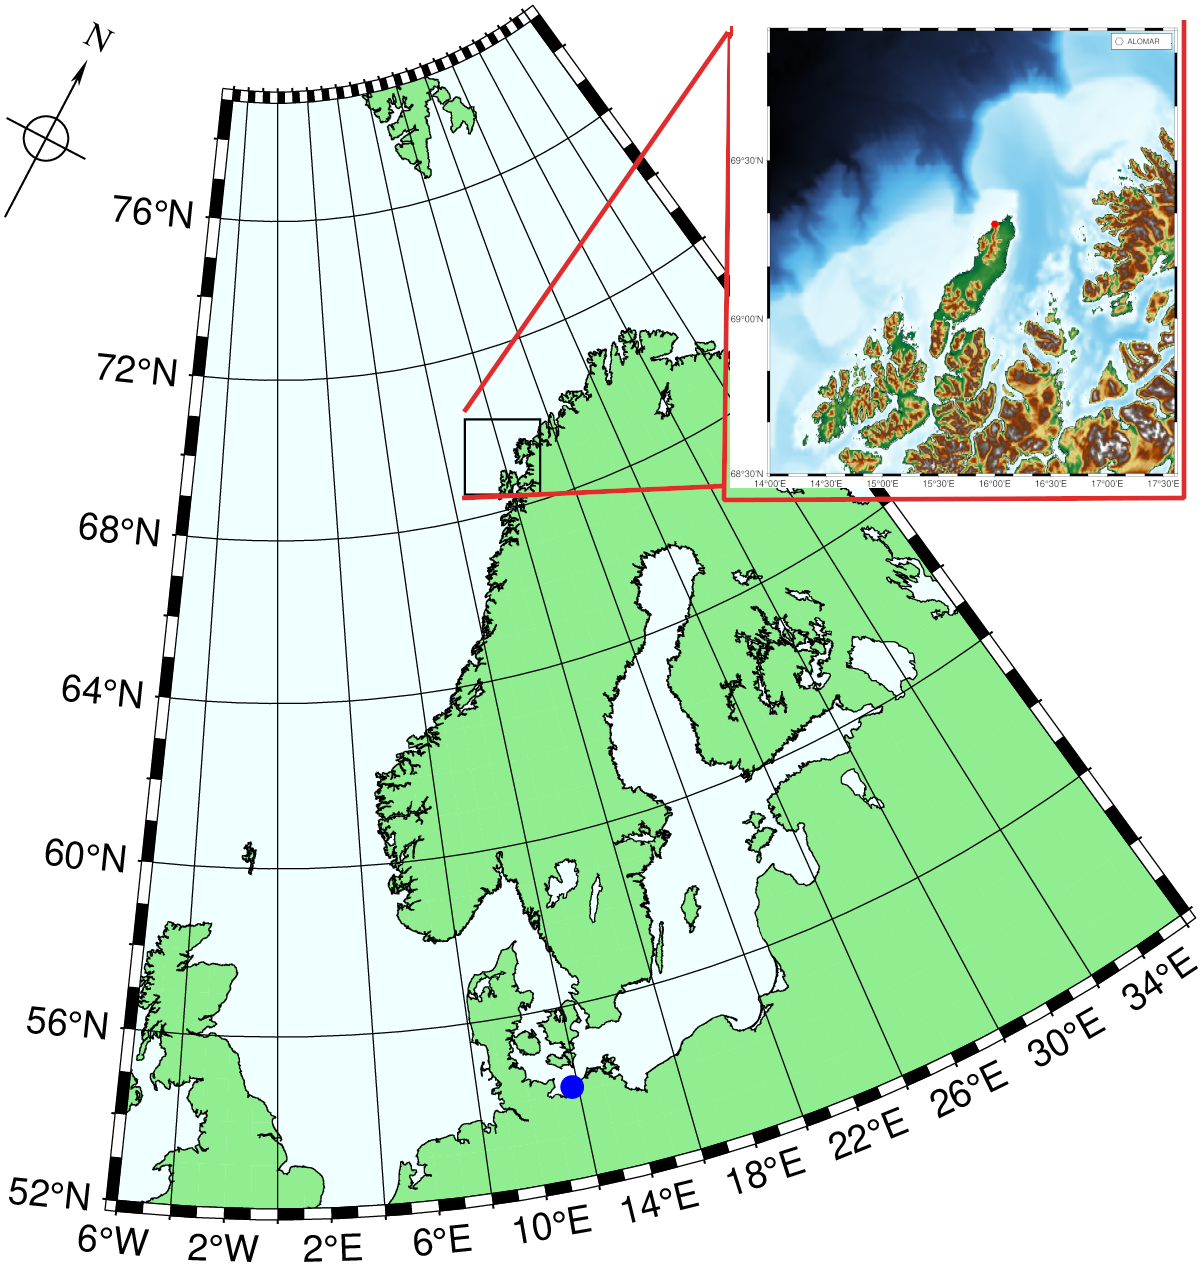
\includegraphics[width=.39\linewidth]{Norway_Andoya_inset.png}\hspace{+3em}
		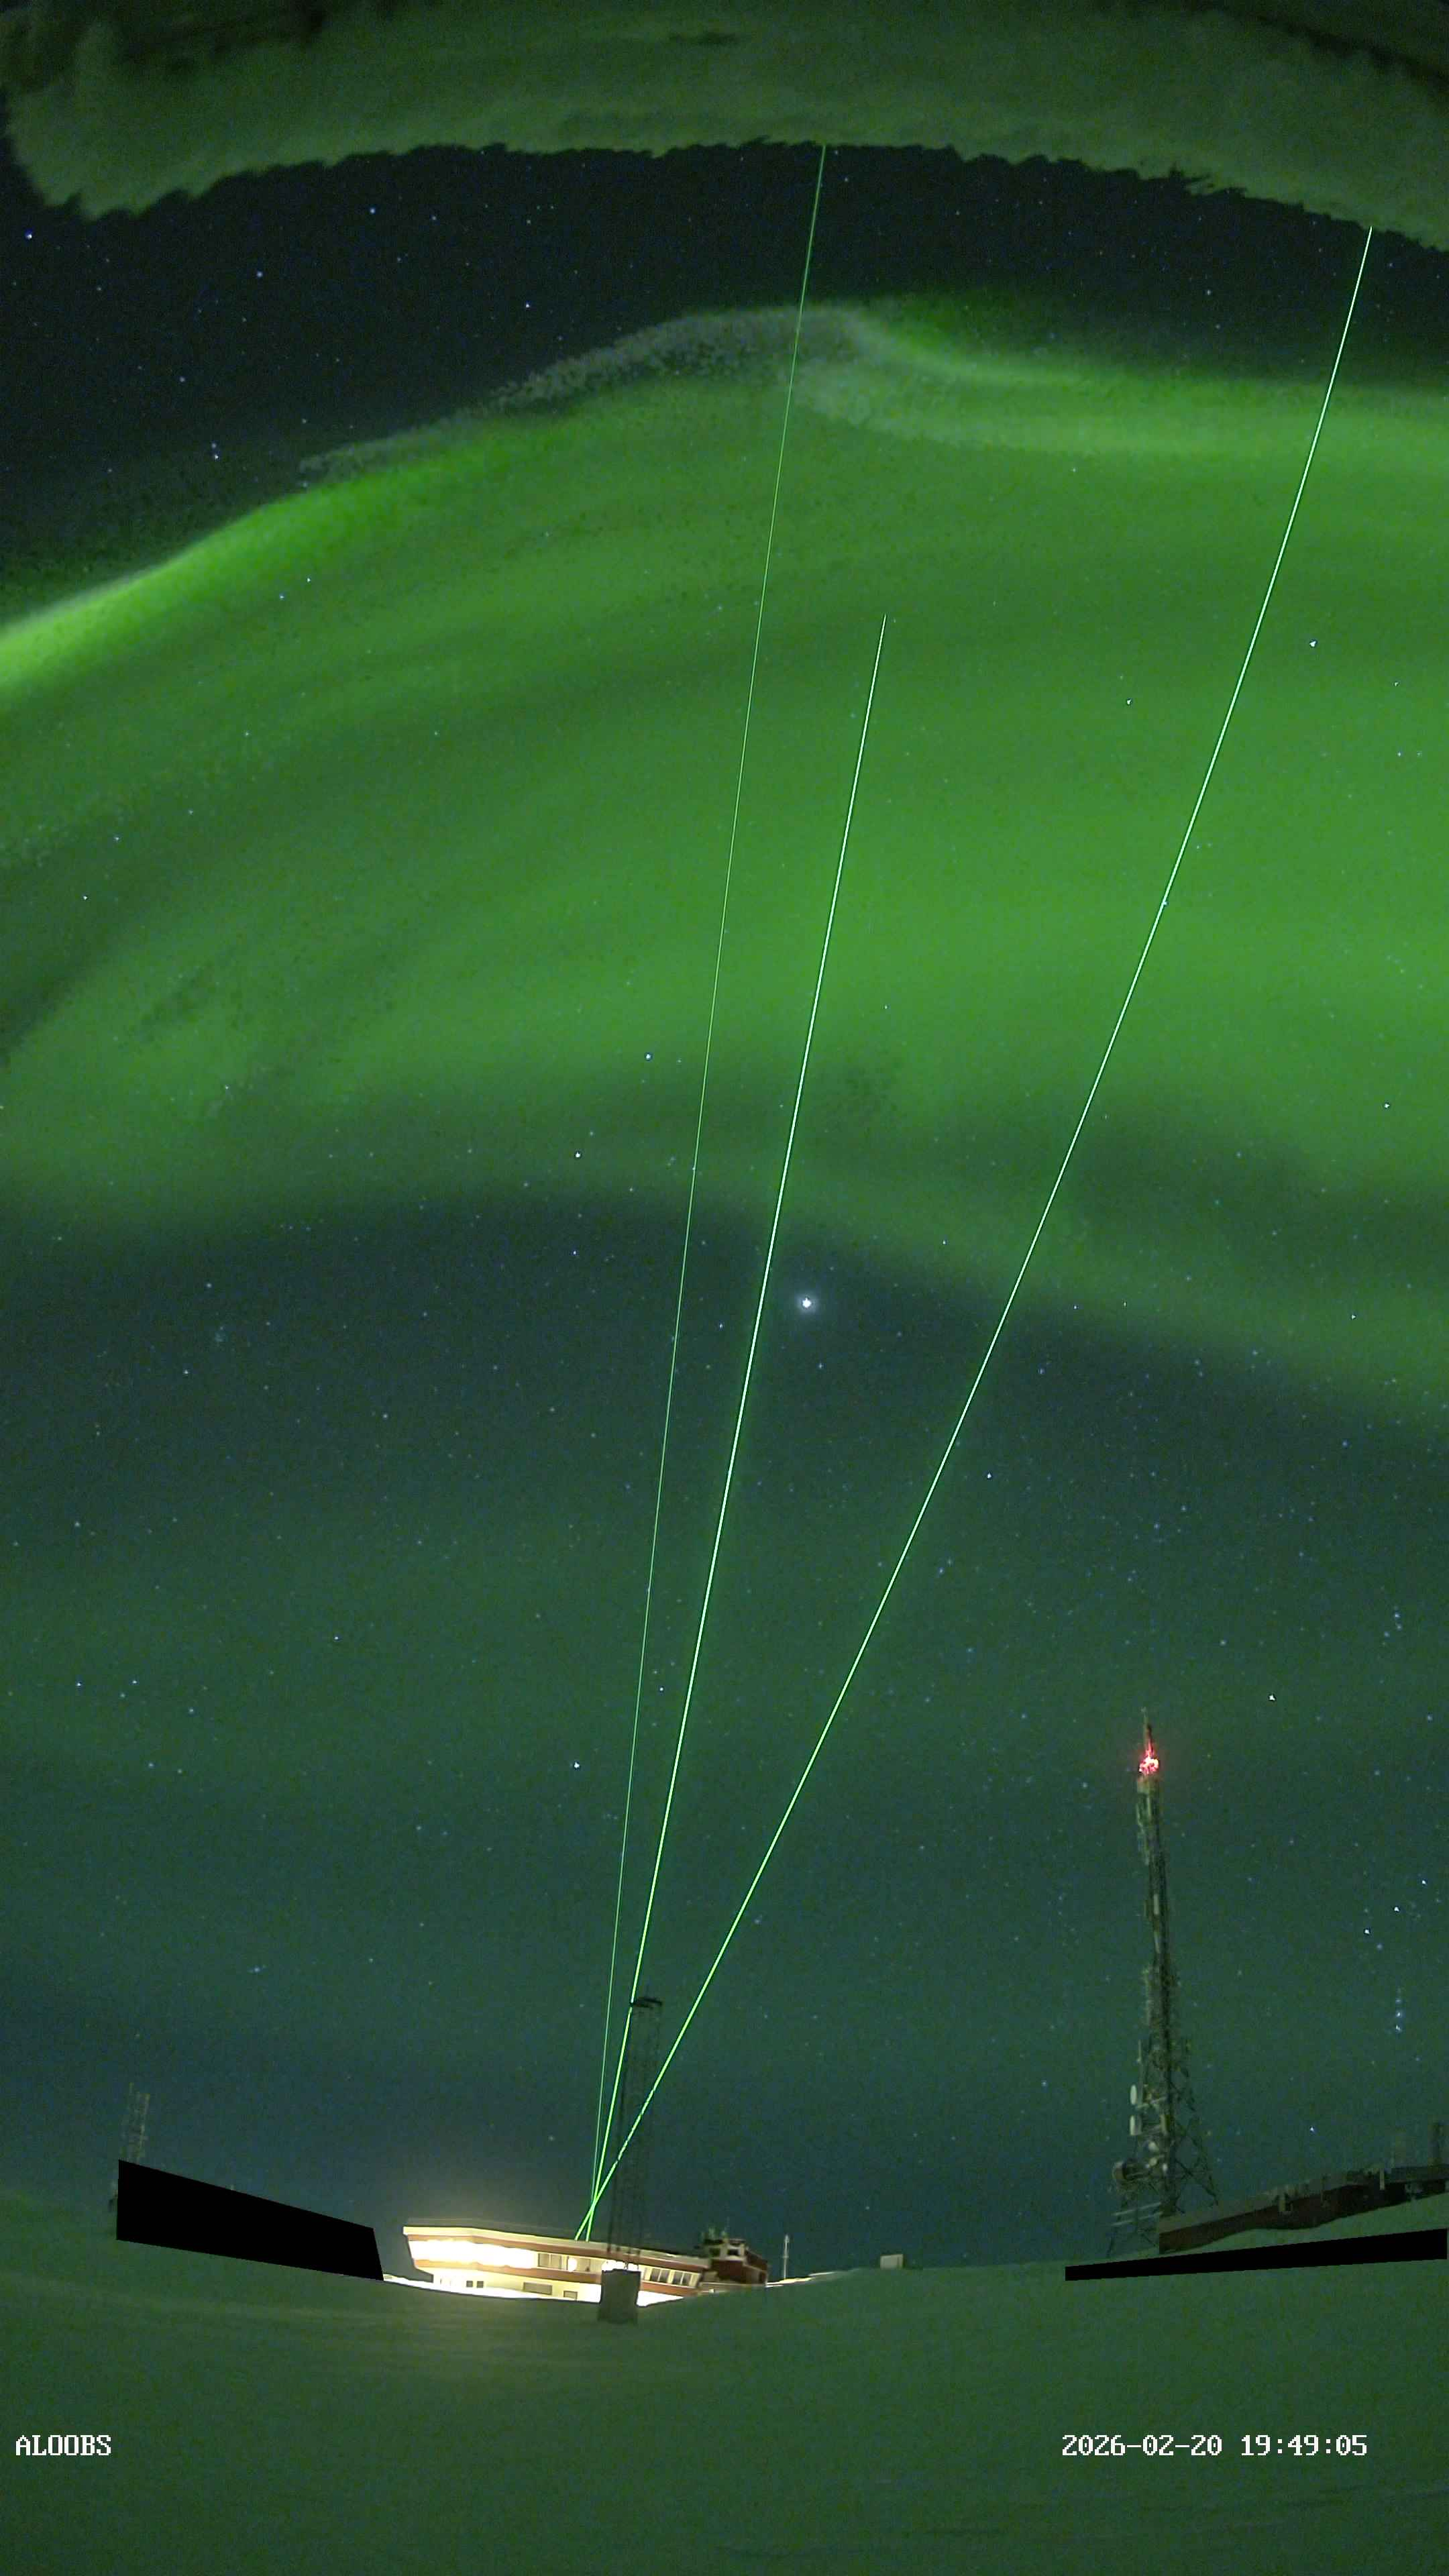
\includegraphics[width=.39\linewidth]{last0023.jpg}%}
	\captionsetup{width=0.8\linewidth} %\small 
	\captionof{figure}{Left: ALOMAR location in Andenes, Norway. Right: Observatory view from 20th~Feb.~2026, note the green laser beams are ALOMAR's RMR and tropospheric lidars, while \euliaa beans at 770~nm wavelength are not visible.}
	\label{fig:alomar} 
	%\multicolumn{2}{r}{
		
	%}\\
	%\end{tabular}
	
\end{minipage}\\

{\large The following analysis is performed using wintertime observations by the \euliaa lidar from its 3 FOV to retrieve particle backscatter coefficient as well as depolarization ratio to characterize the signature from aerosols and high-altitude clouds.
}
%\colouredcircle Sea ice - atmosphere coupling conceptual model\\


} % end of box

%%%%%%%%%%%%%%%%%%%%%%%%%%%%%%%%%%%%%%%%%%%%%%%%%%%%%%%%%%%%%%%%%%%%%%%%%%%%%%
  \headerbox{3.- Stratospheric Aerosols and Clouds during wintertime 2025-2026}{name=results,column=1,row=0,span=3}{
%%%%%%%%%%%%%%%%%%%%%%%%%%%%%%%%%%%%%%%%%%%%%%%%%%%%%%%%%%%%%%%%%%%%%%%%%%%%%%
{\Large From January 20 to 23, 2026 a significant presence of stratospheric aerosols in the Junge layer, approximately located at altitudes between 15 and 25~km, together with the passage of Polar stratospheric clouds have been observed almost continuously.}\\
\vspace{+1.5em}
\begin{minipage}{0.92\linewidth}
	\begin{tabular}{cccc||r} %{@{}lcr@{}}
		\multicolumn{4}{l}{\vspace{+1em}\colouredcircle {\large \euliaa measured wind, particle backscatter coefficient, depolarization ratio, and temperature during this event.\hfill}} & \\
		%\textbf{\Large COUPLED}	& \textbf{\Large DECOUPLED} \\
		% Row with zenith BSC:
		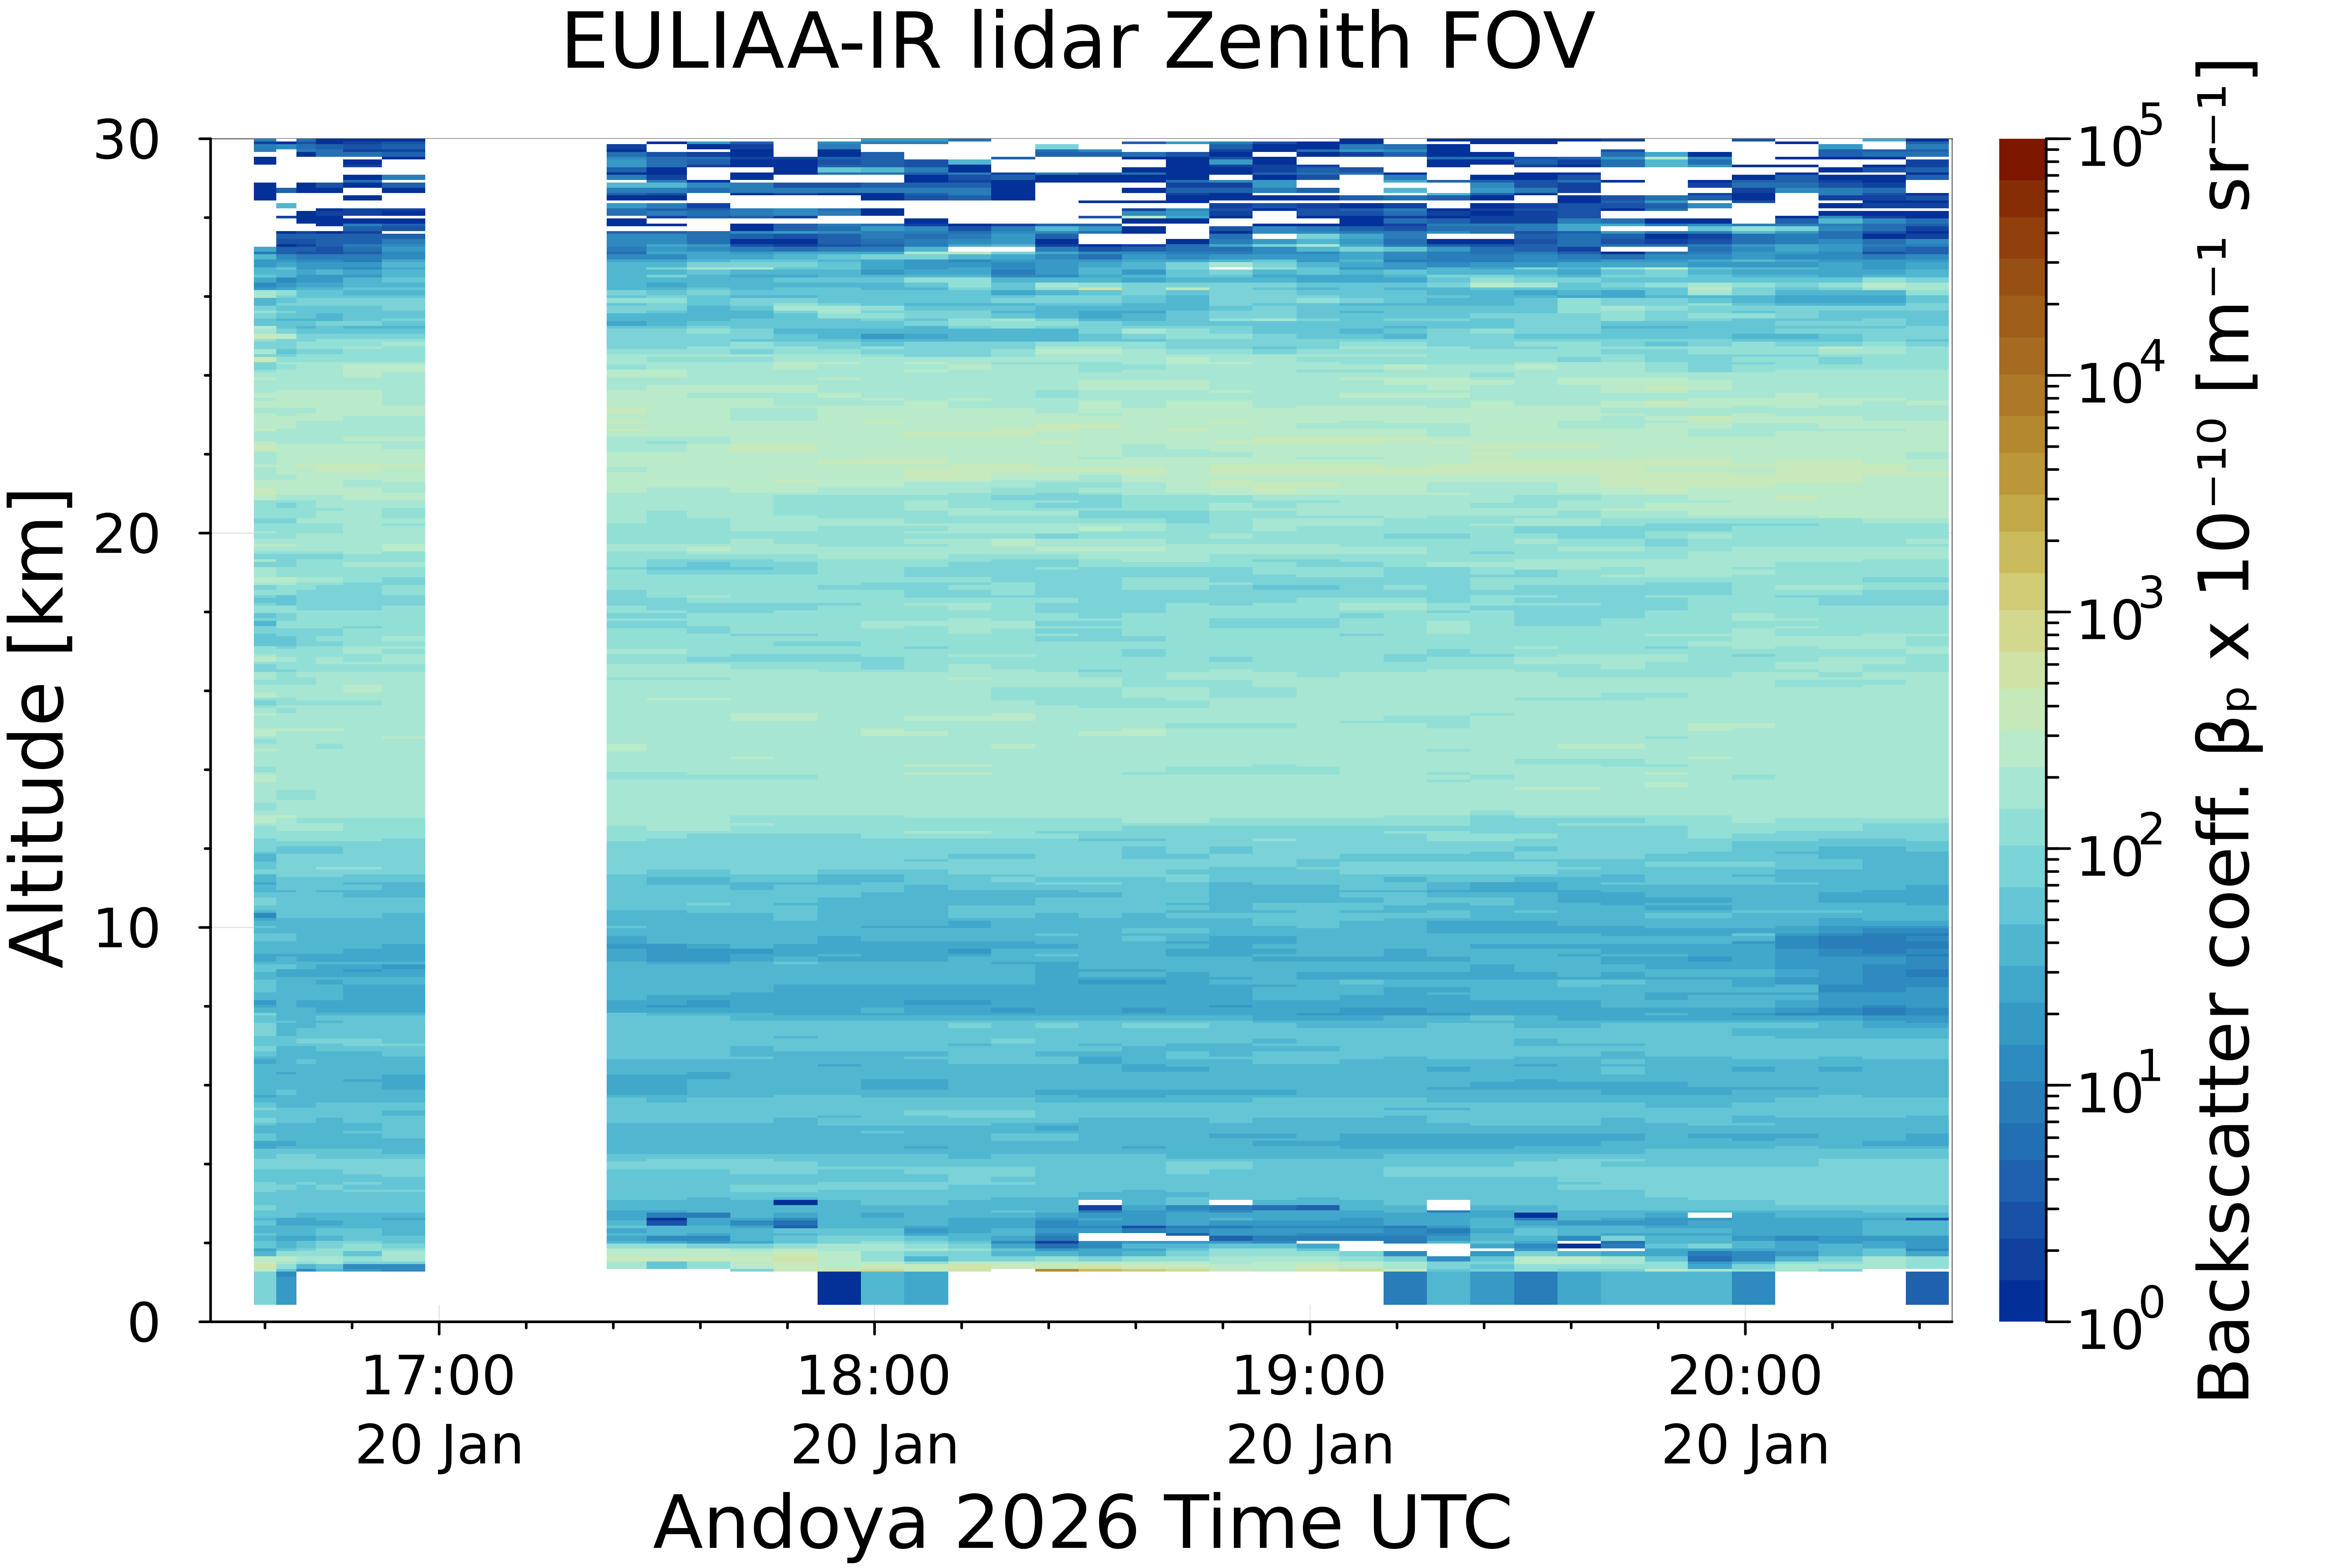
\includegraphics[width=.20\linewidth]{EULIAA_L1_2026-01-20_16-36-00_dT15min_dH200m_OL_BSC_ZFOV_17_00_20_00.png} &
		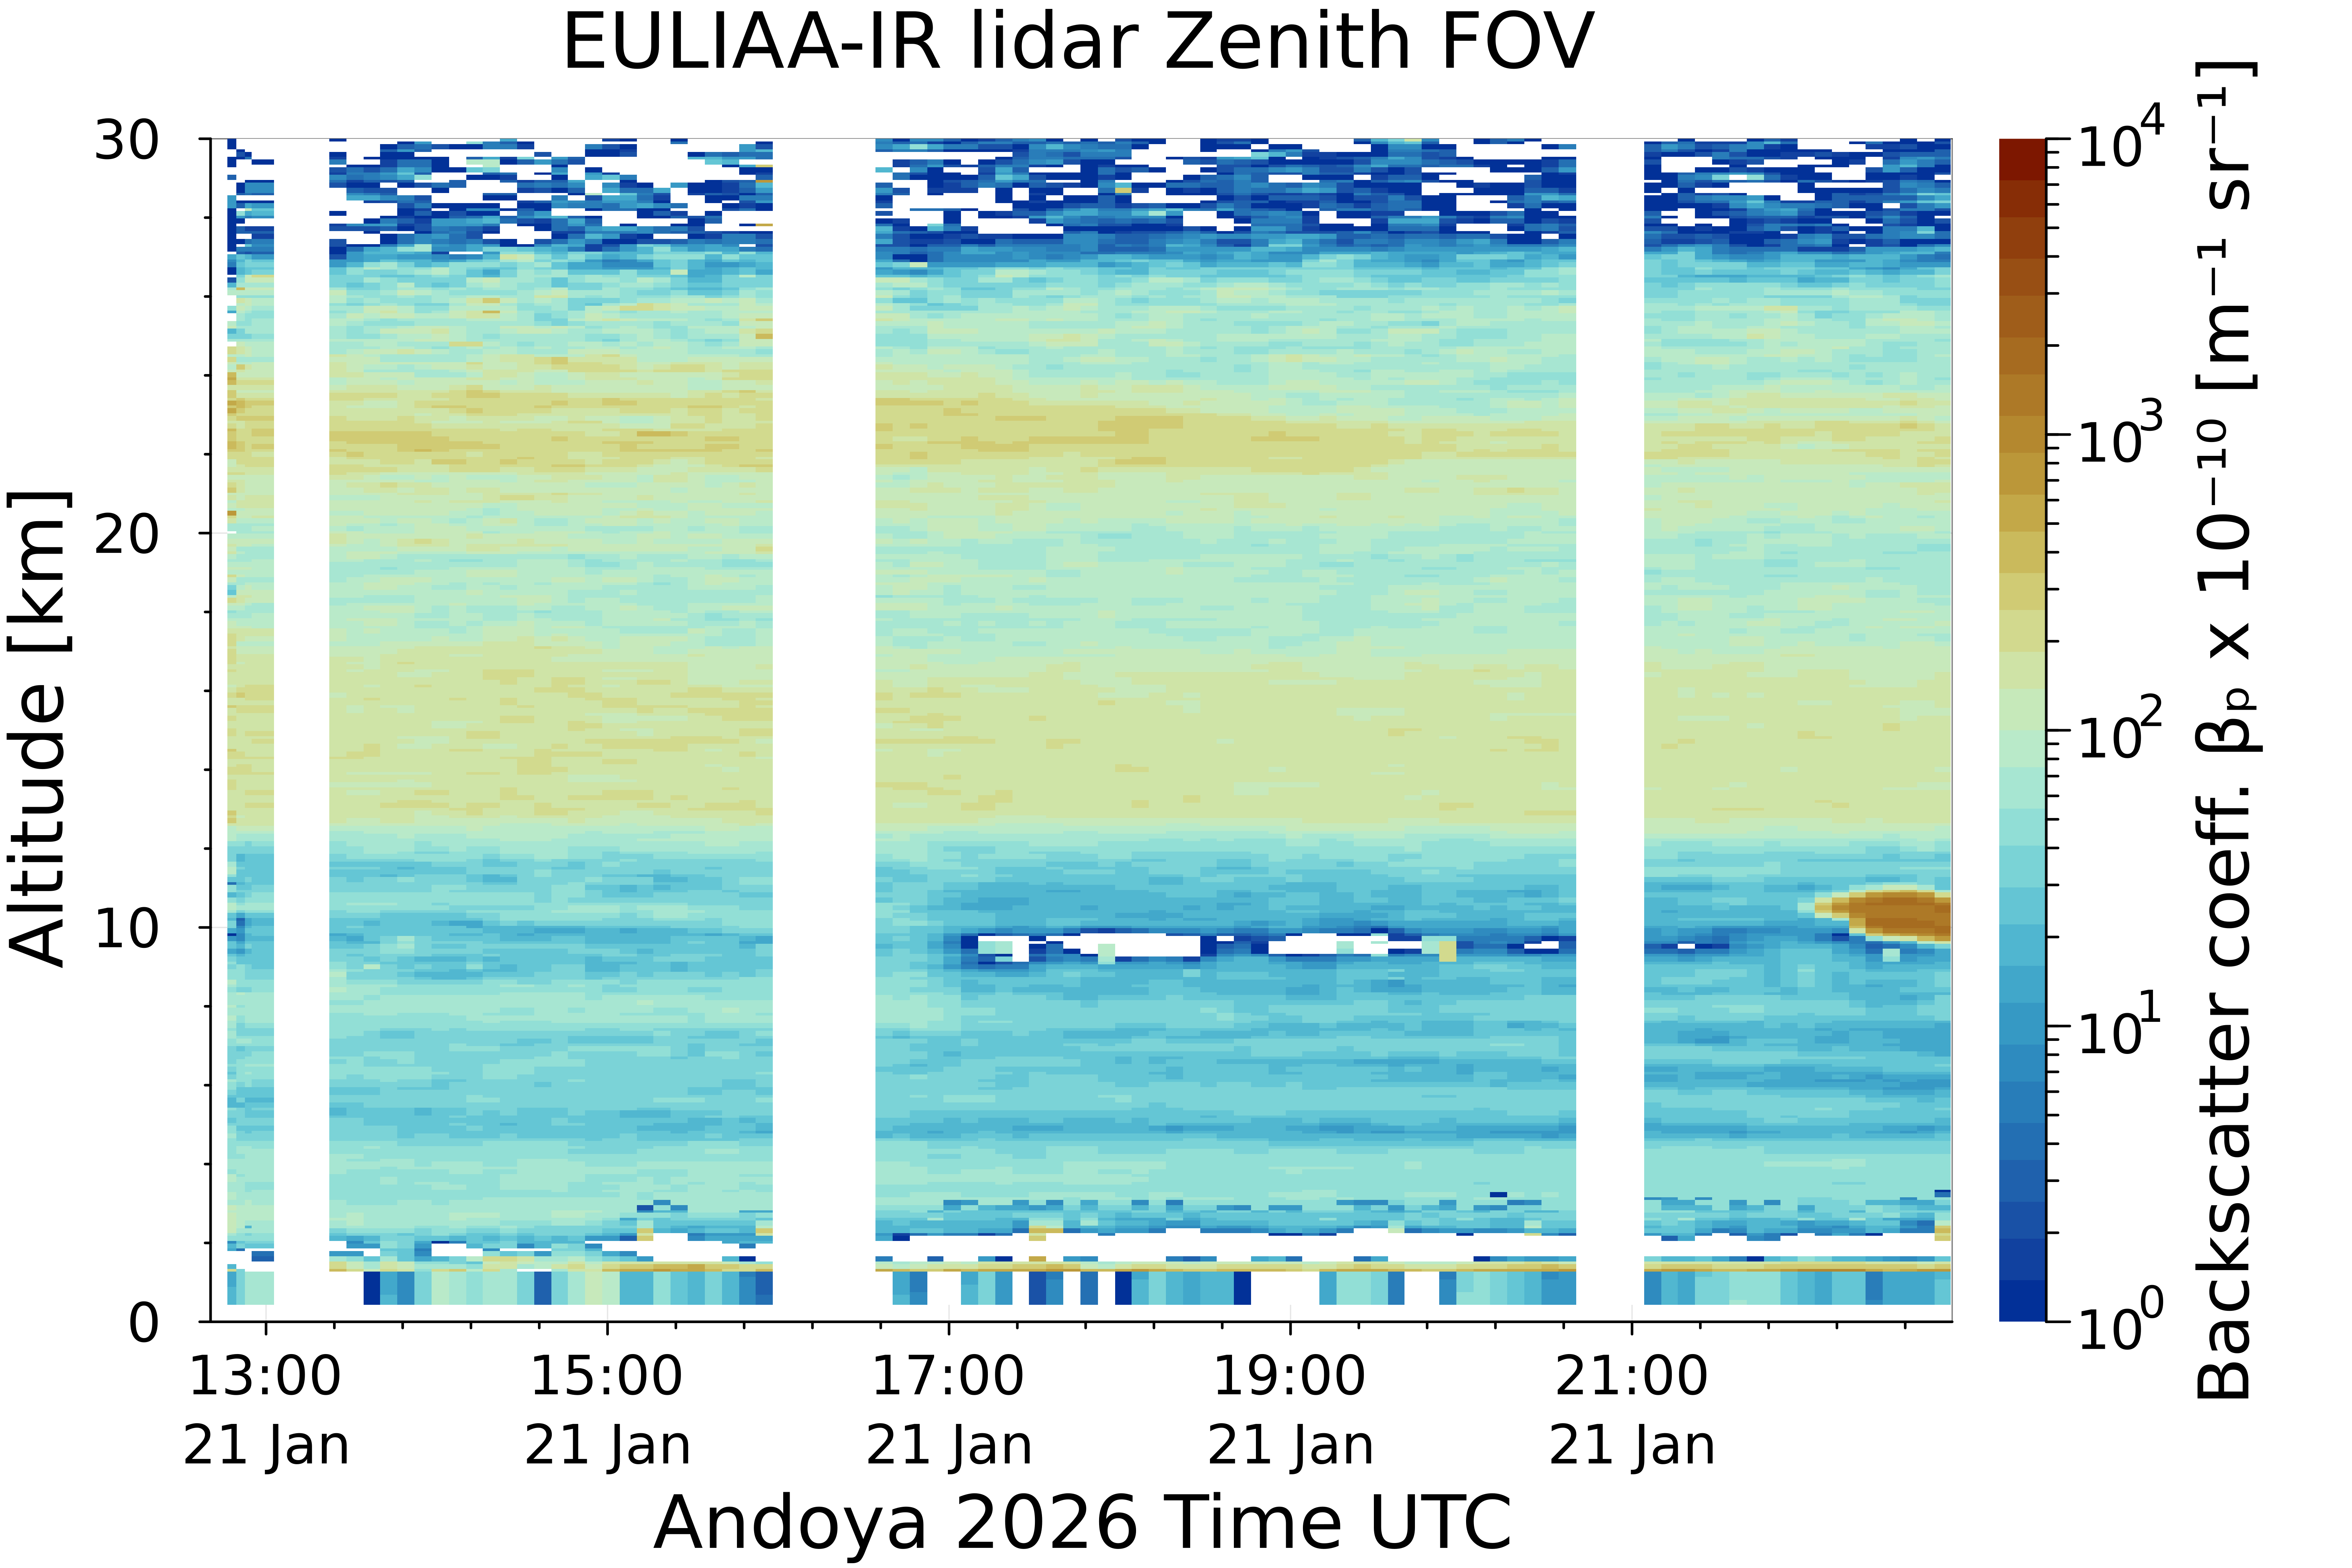
\includegraphics[width=.20\linewidth]{EULIAA_L1_2026-01-21_12-48-00_dT15min_dH200m_OL_BSC_ZFOV_13_00_21_00.png} &
		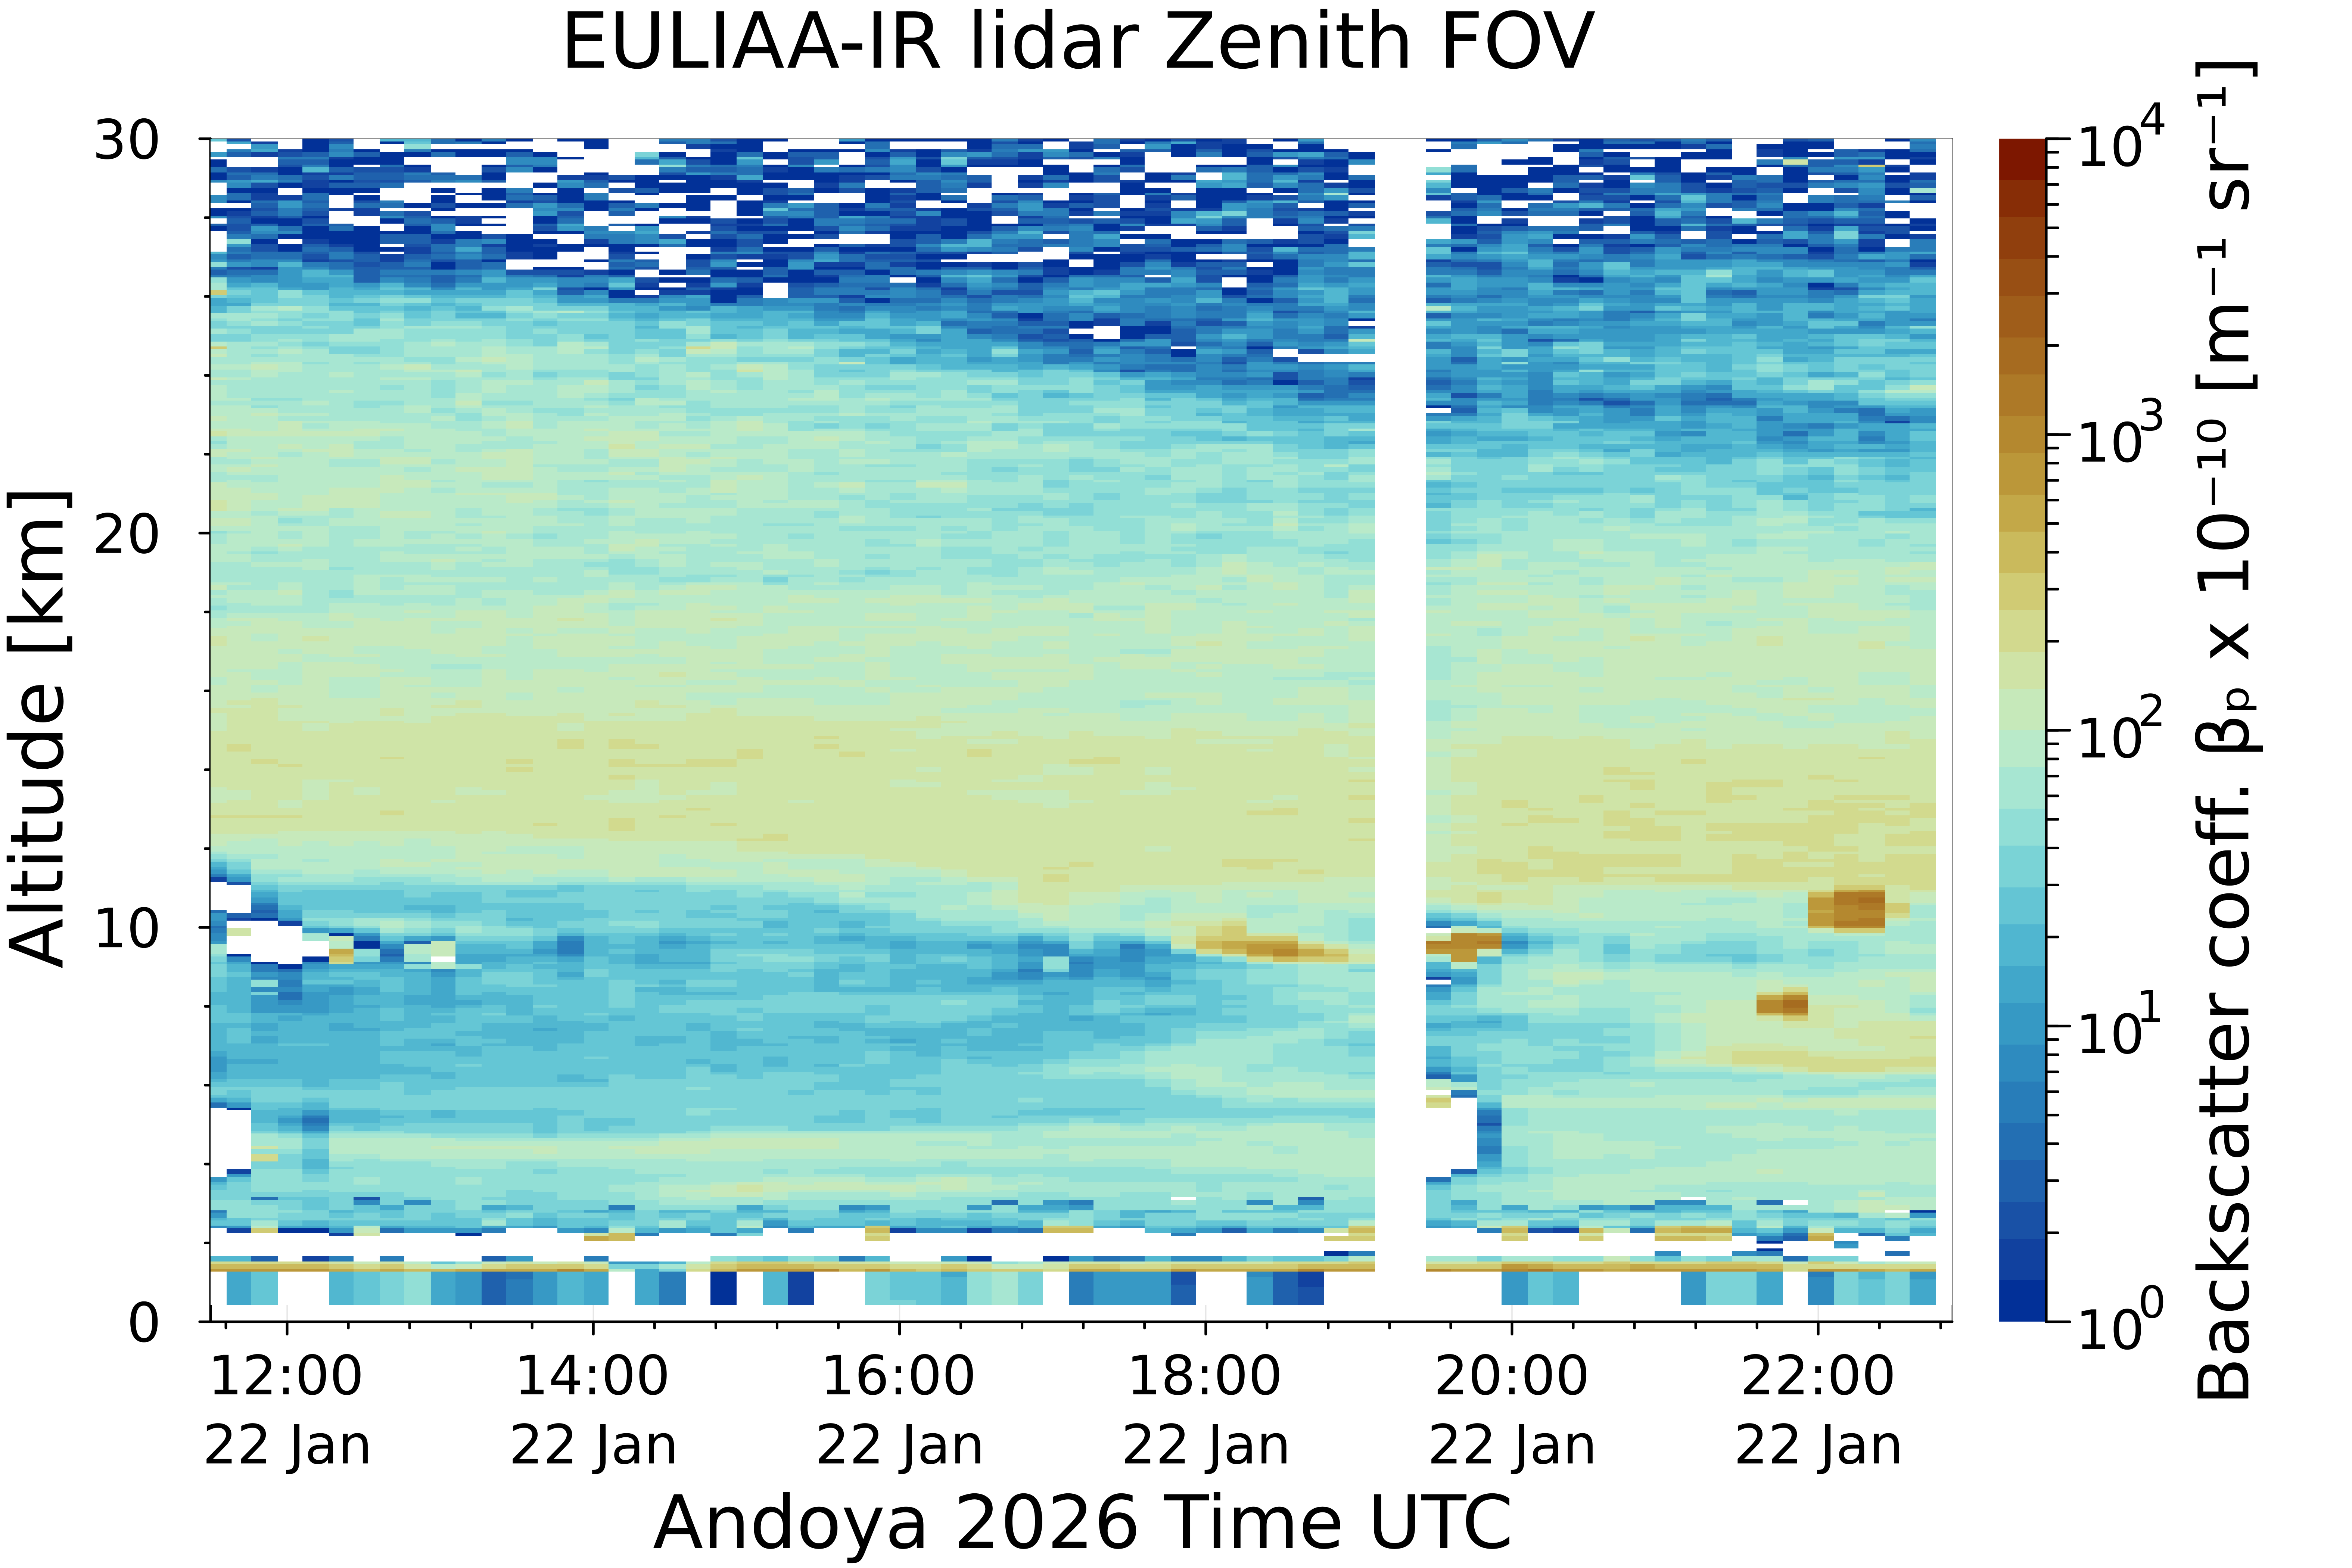
\includegraphics[width=.20\linewidth]{EULIAA_L1_2026-01-22_00-00-00_dT15min_dH200m_OL_BSC_ZFOV_12_00_22_00.png} &
		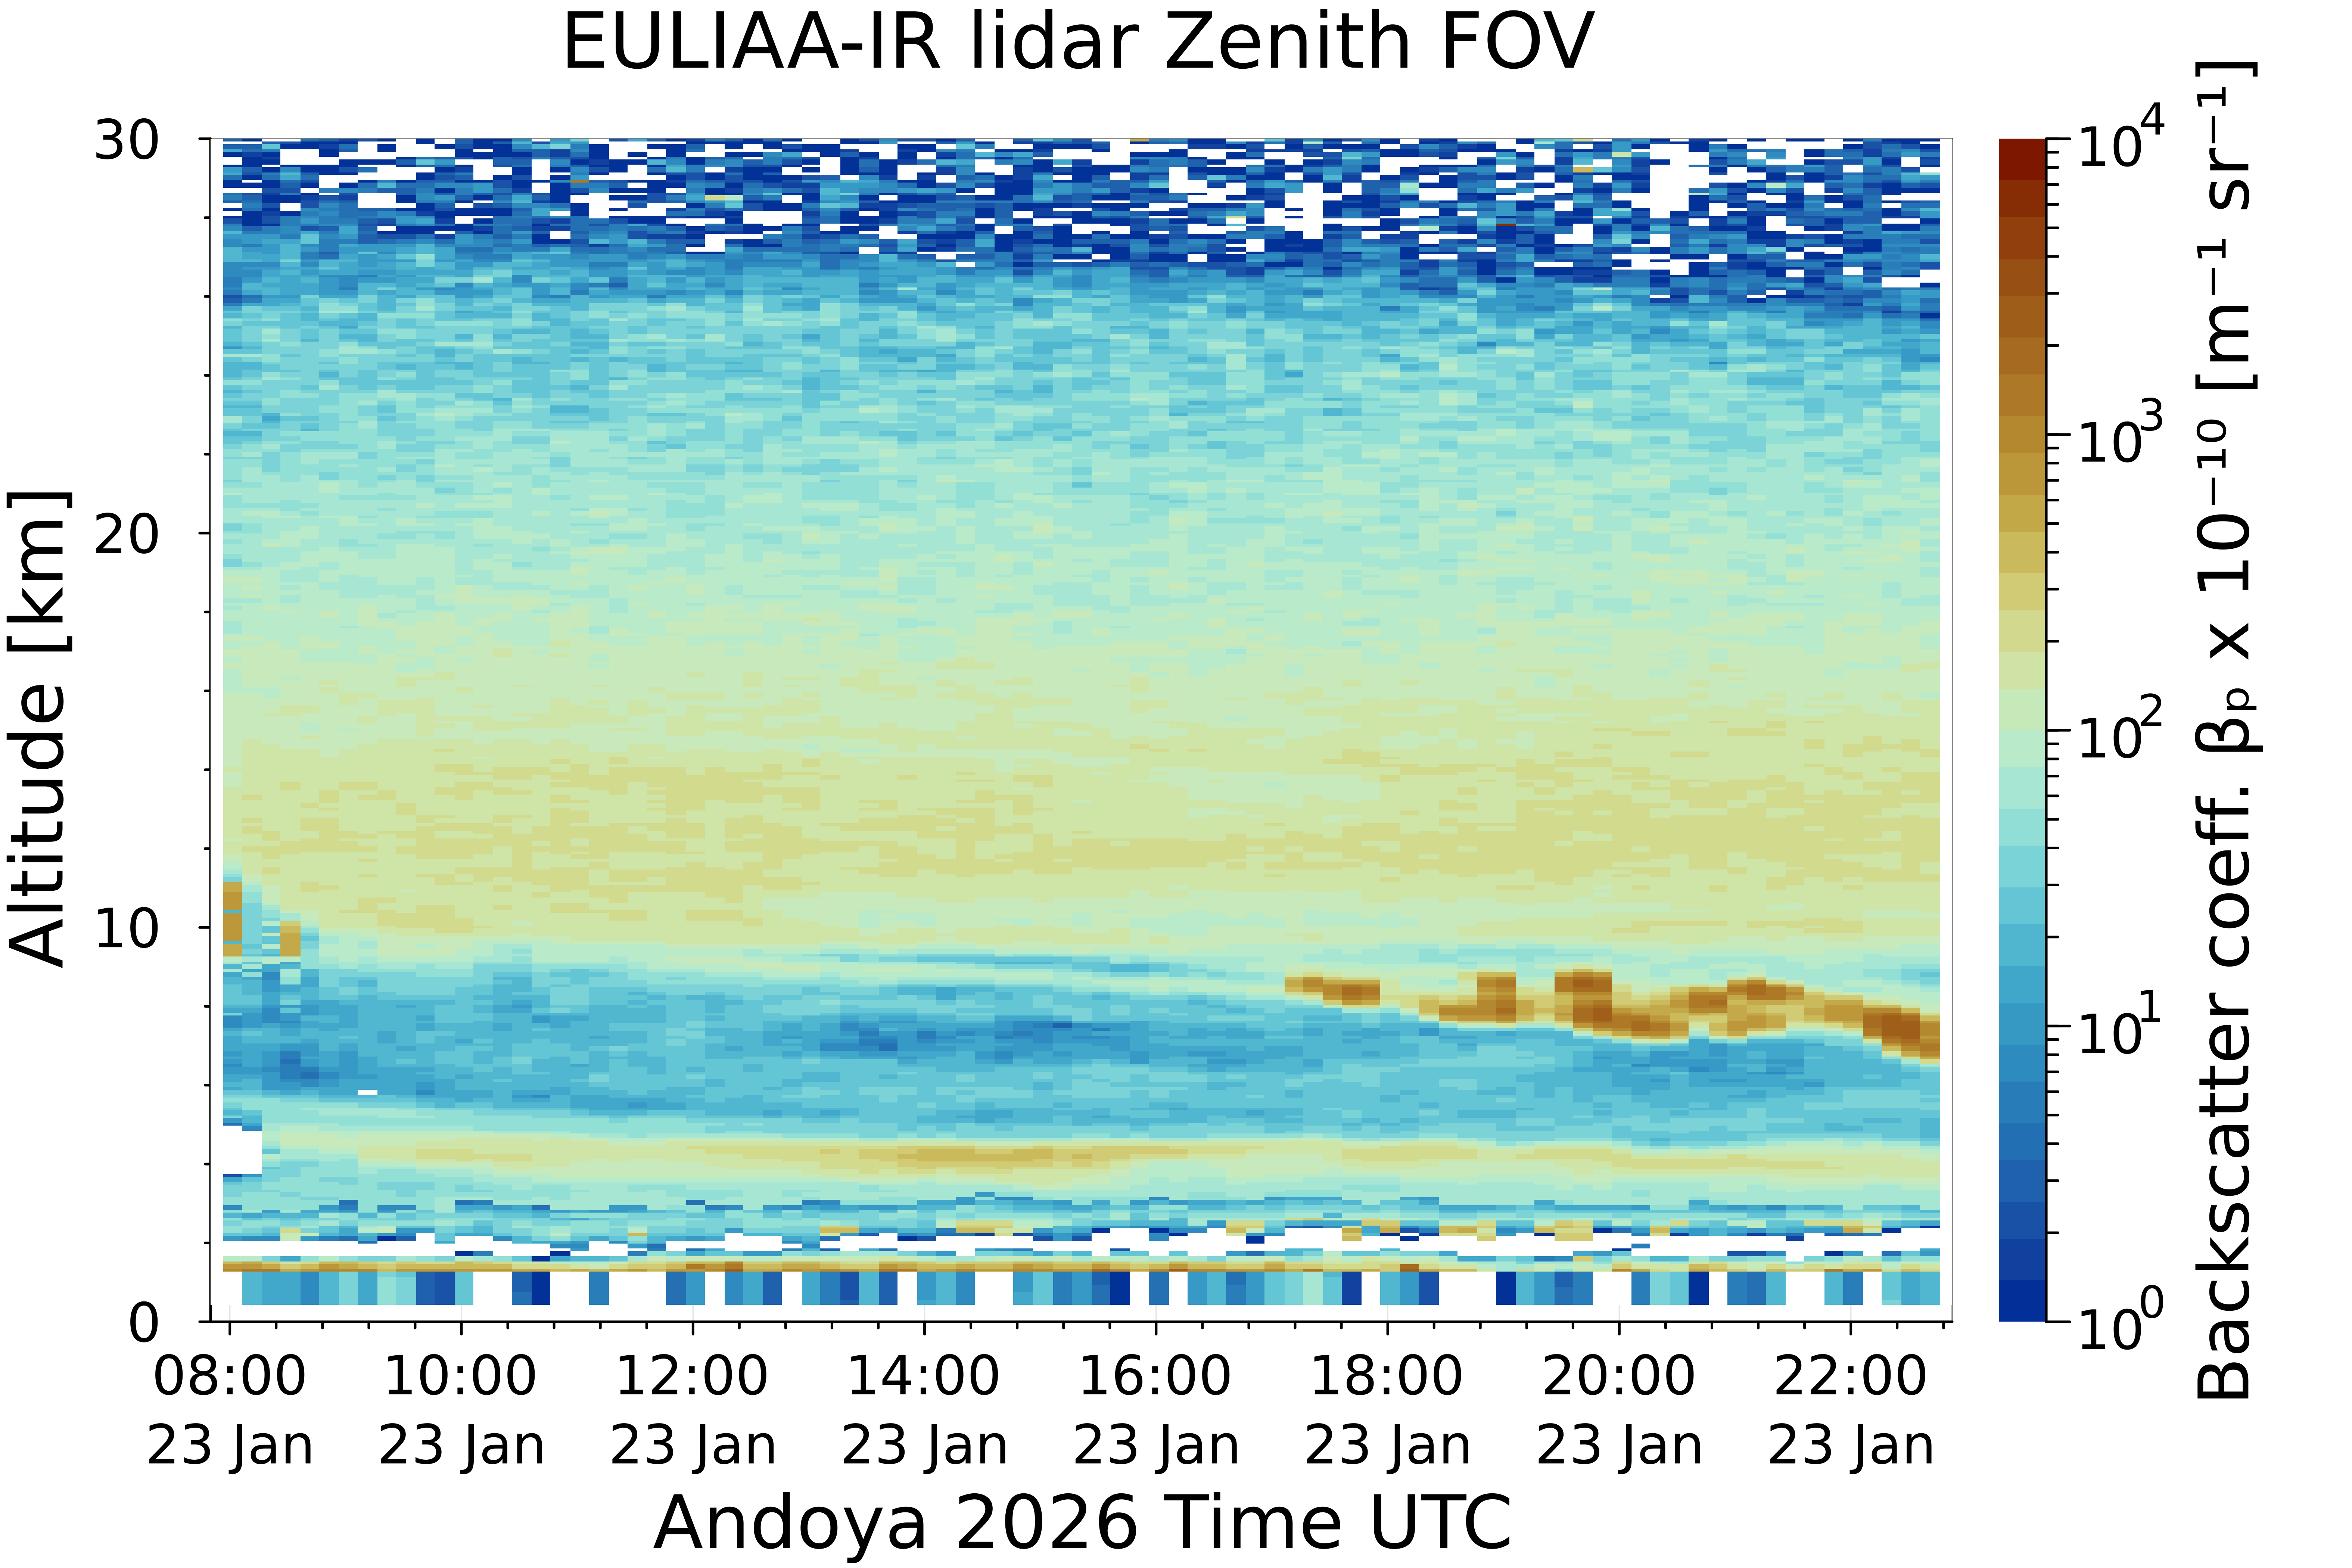
\includegraphics[width=.20\linewidth]{EULIAA_L1_2026-01-23_00-00-00_dT15min_dH200m_OL_BSC_ZFOV_08_00_22_00.png} &
		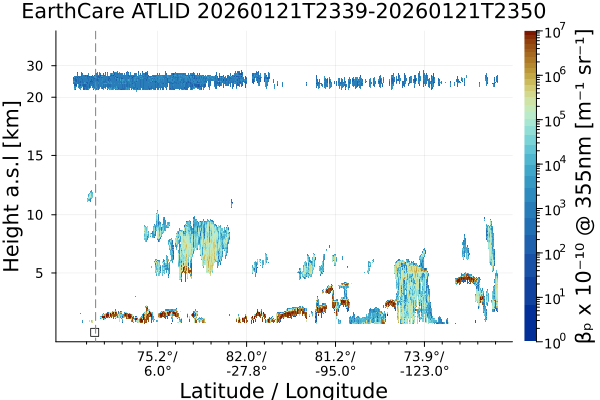
\includegraphics[width=.20\linewidth]{EarthCare_ATLID_20260121T2339-20260121T2350_backsct.png}
		\\
		
		% Row with BSC off-zenith FOV:
		\hfill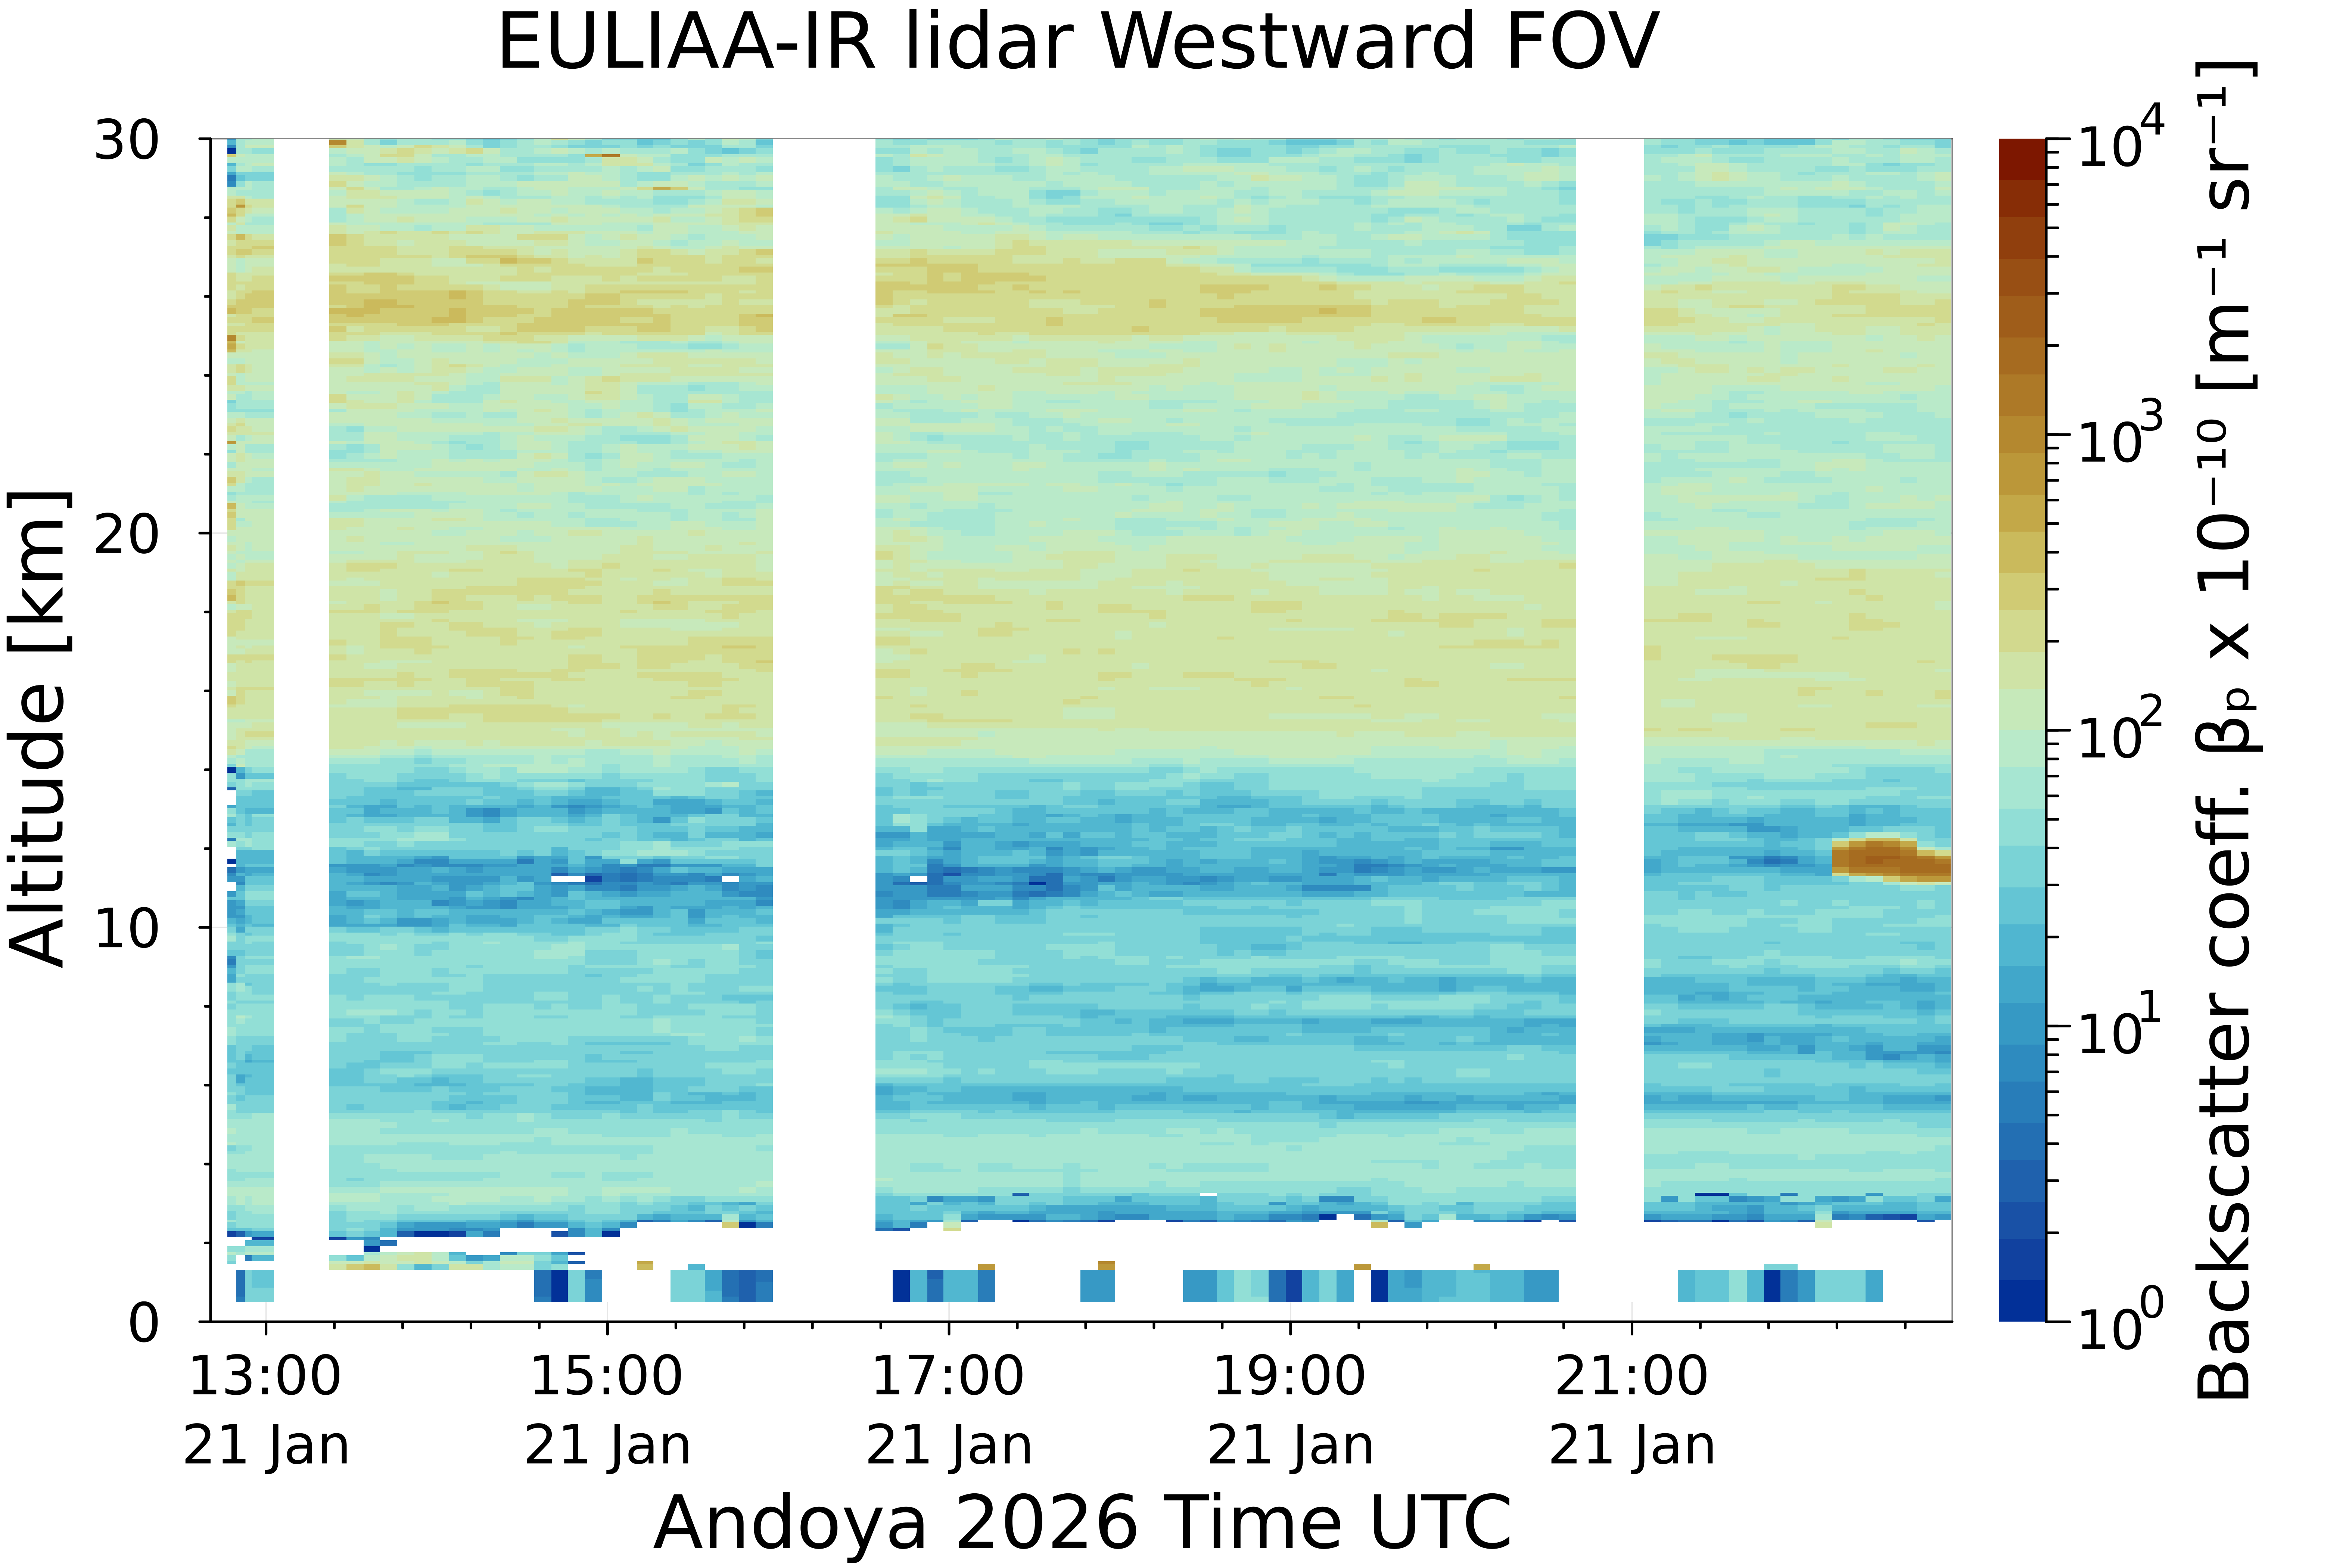
\includegraphics[width=.20\linewidth]{EULIAA_L1_2026-01-21_12-48-00_dT15min_dH200m_OL_BSC_EFOV_13_00_21_00.png} &
		\begin{minipage}{0.18\linewidth}
			\vspace{-12em}
			\centering
			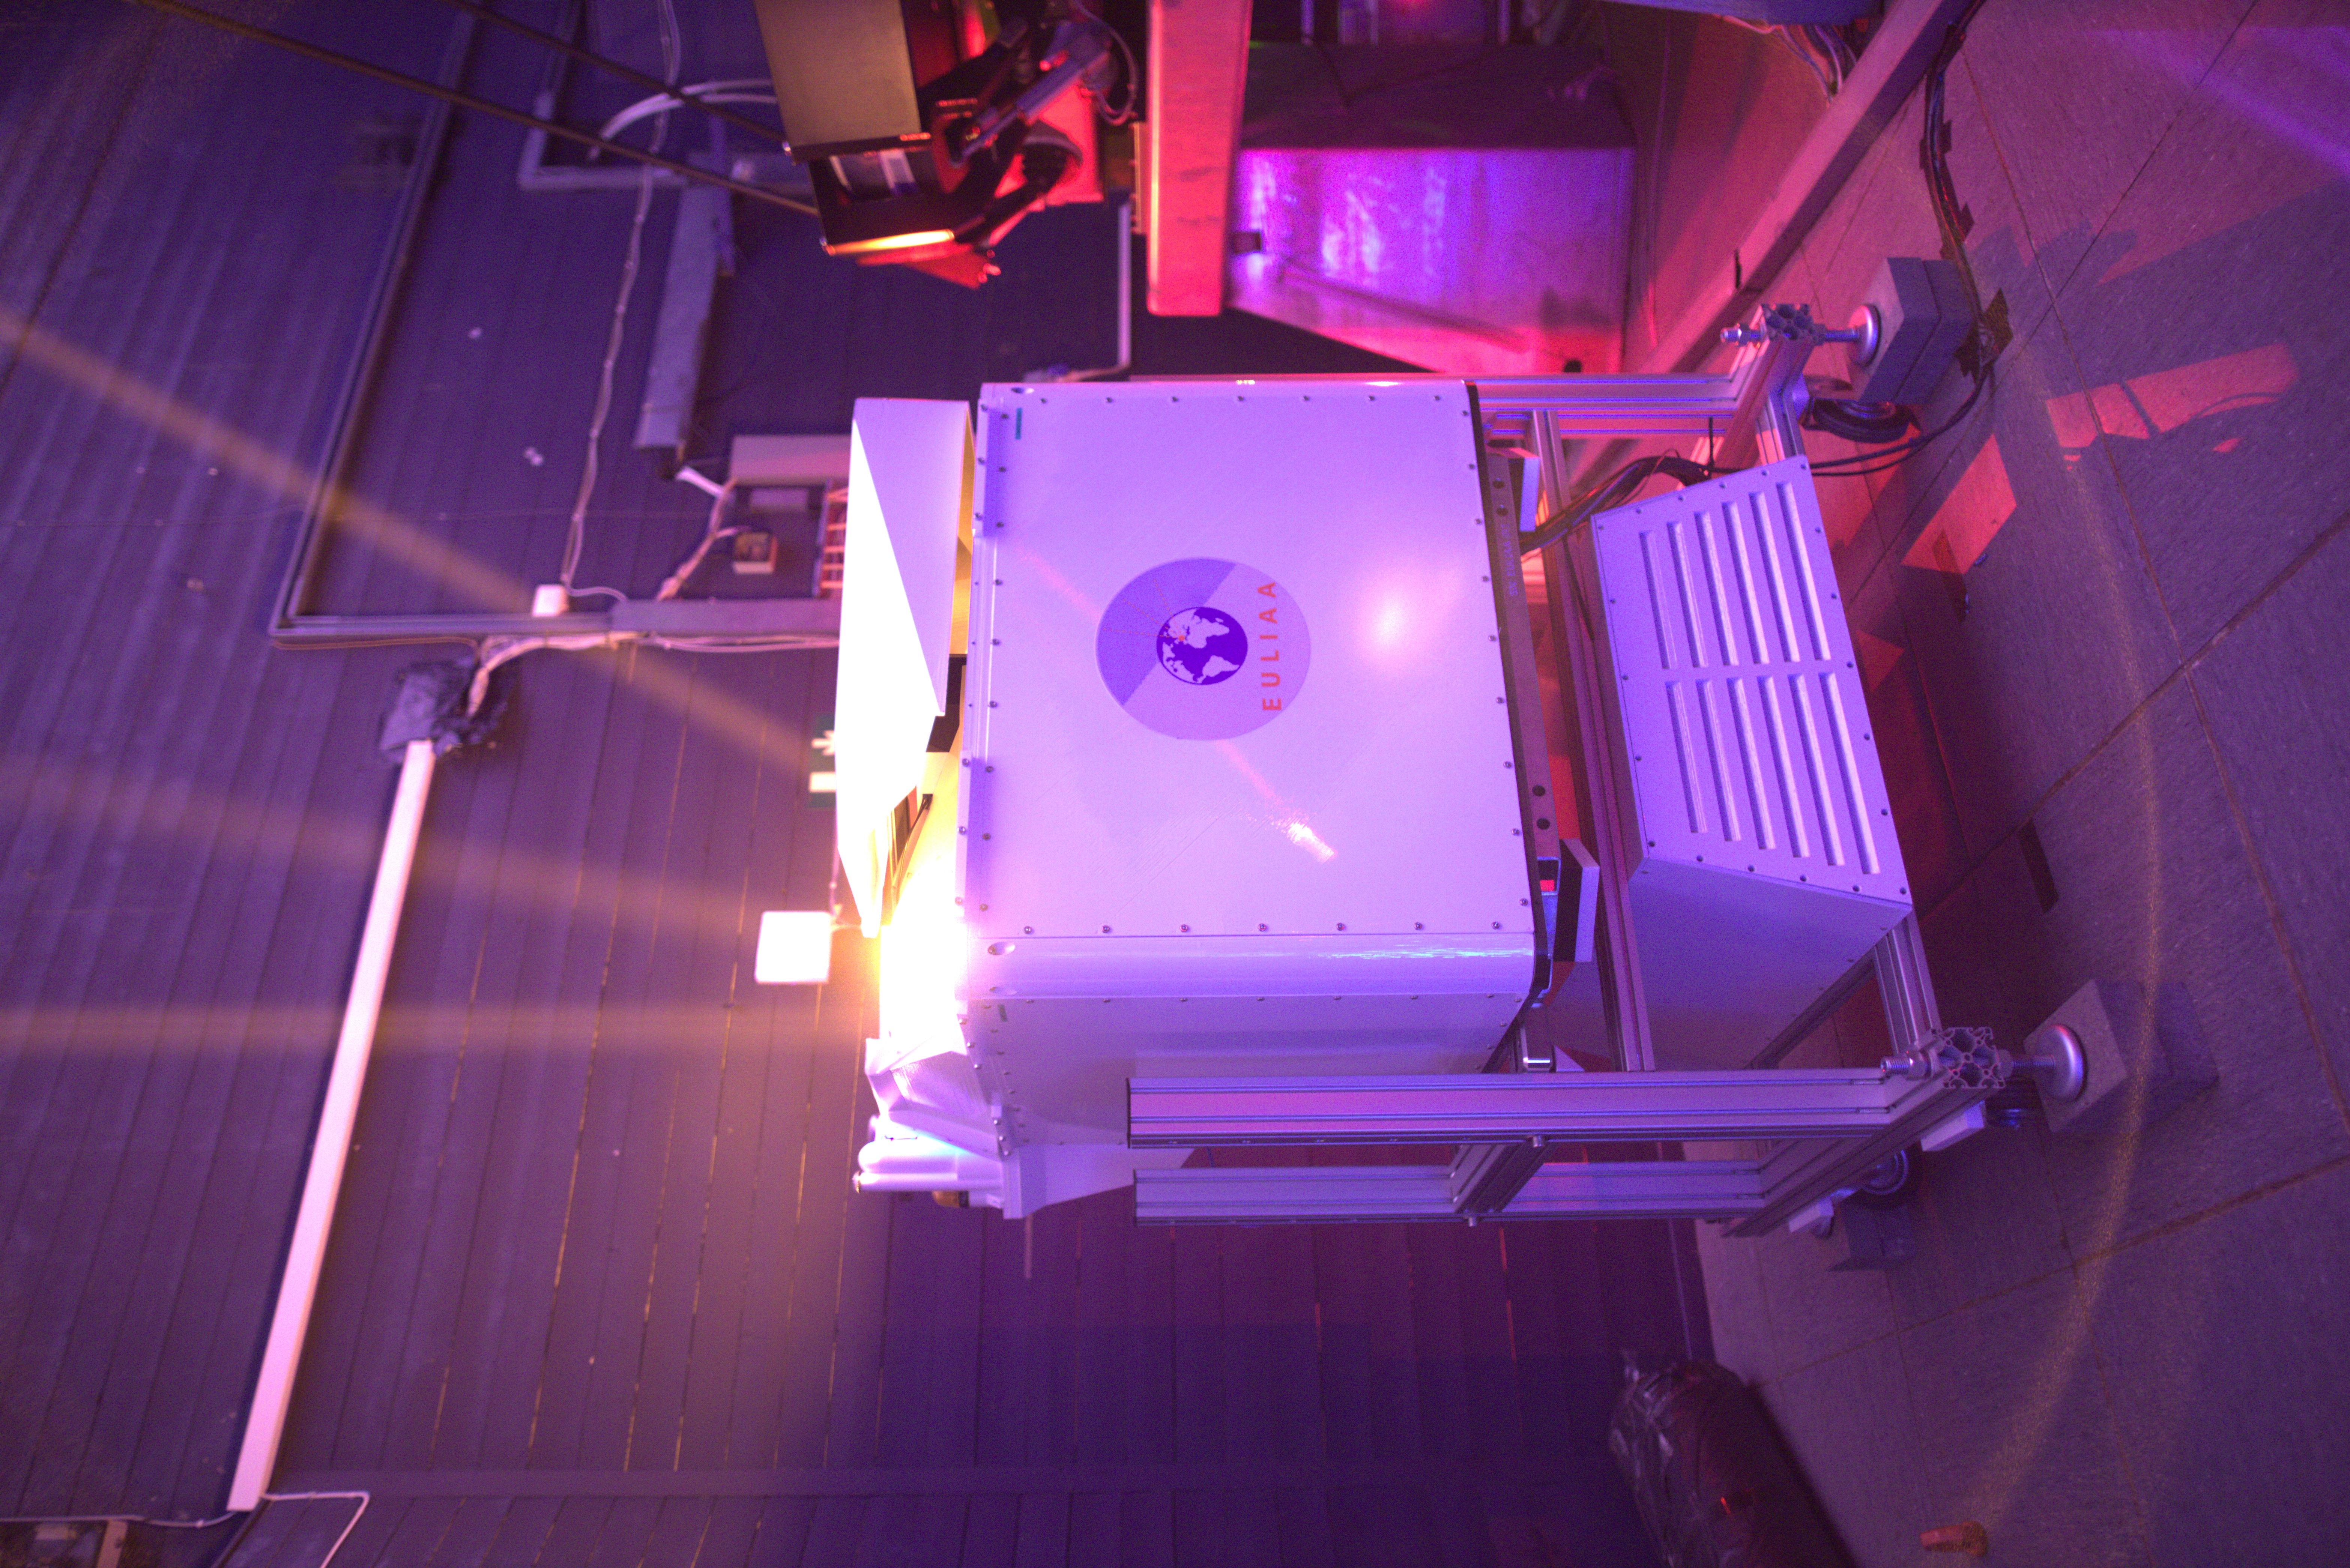
\includegraphics[width=.48\linewidth]{EULIAA_IR1_Andenes.png}	
		\end{minipage} &
		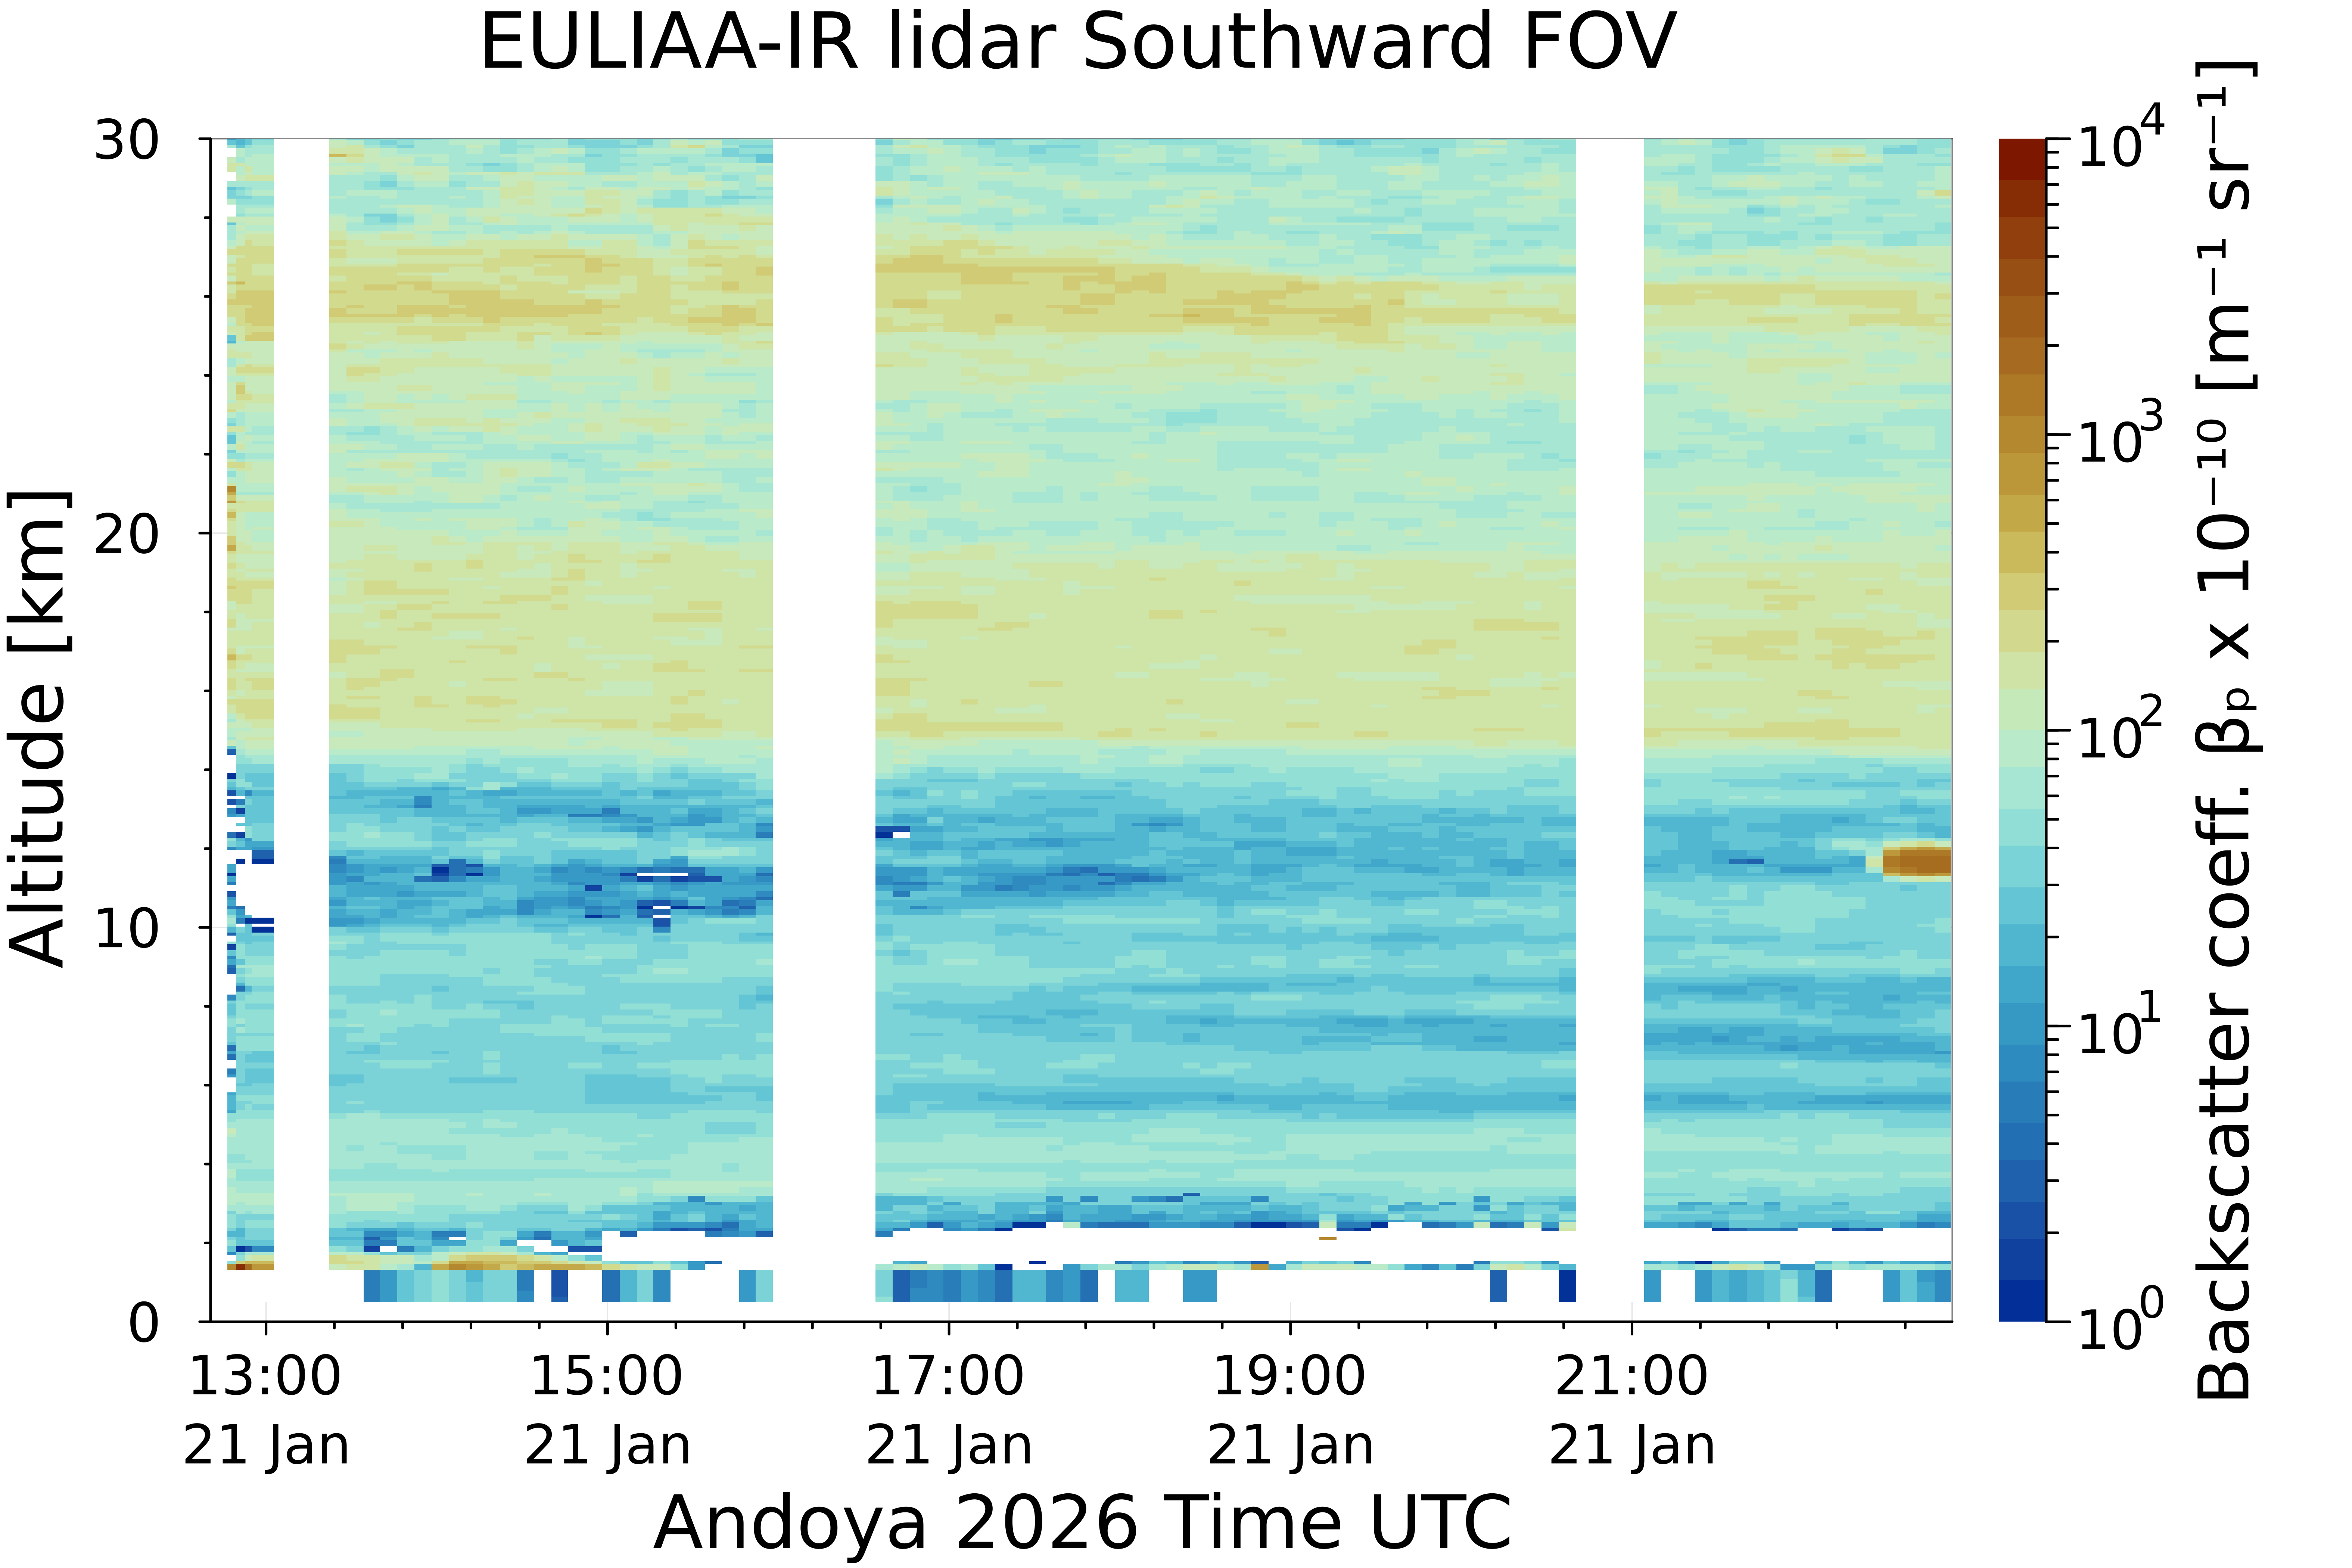
\includegraphics[width=.22\linewidth]{EULIAA_L1_2026-01-21_12-48-00_dT15min_dH200m_OL_BSC_NFOV_13_00_21_00.png} &
		\begin{minipage}{0.18\linewidth}
			\vspace{-12em}
			{ The \euliaa lidar ($\leftarrowtail$ middle picture left) measures $\beta_p$ at 3 FOV, in ALOMAR one 30$^\circ$ off-zenith FOV westwards and southwards, one zenith with depolarization. That gives the opportunity to observe the dynamic of the atmosphere by retrieving the wind and $\beta_p$ off-zenith as well ($\leftarrowtail$ two plots next to \euliaa picture).\\
				The sequence of corresponding depolarization ratio $\delta_\circ$ for this event is shown below $\downarrow$.\vfill}	
		\end{minipage} &
		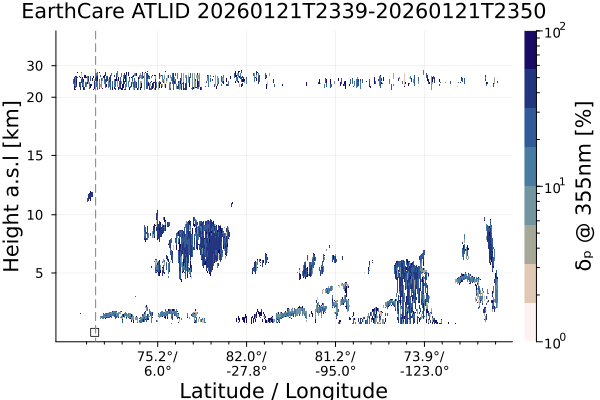
\includegraphics[width=.20\linewidth]{EarthCare_ATLID_20260121T2339-20260121T2350_depol.png}
		\\
		
		% Row with depolarization:
		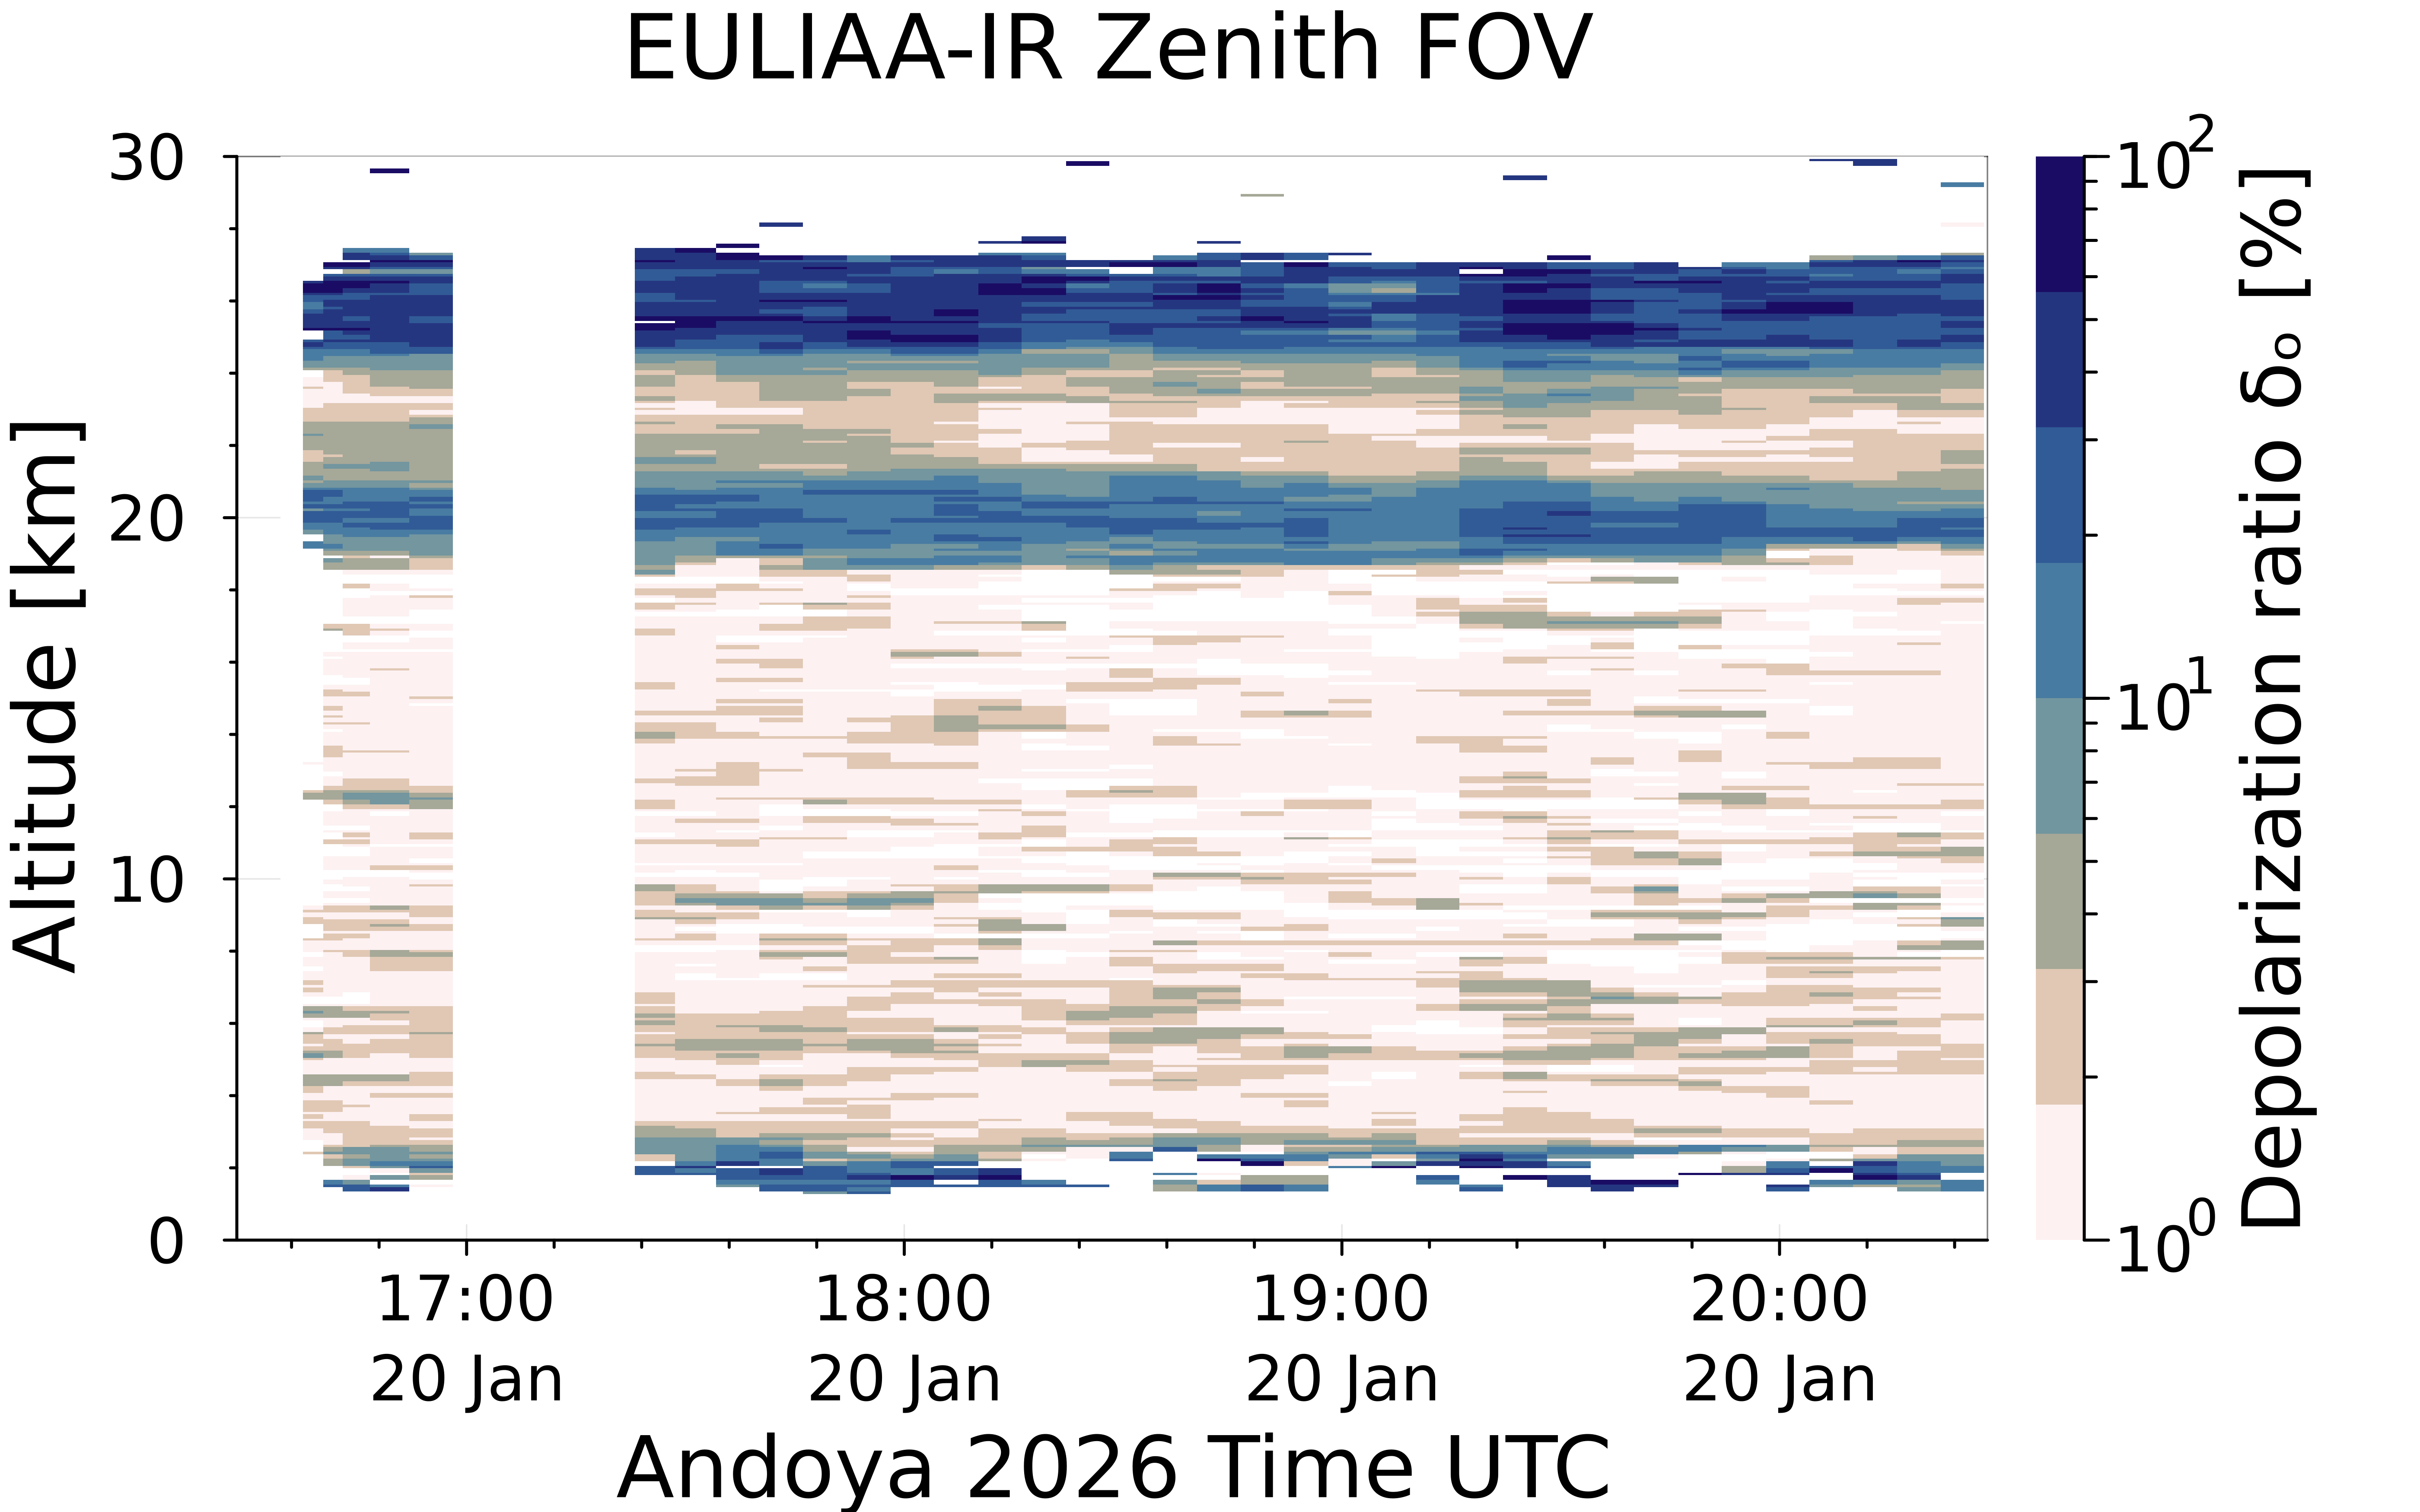
\includegraphics[width=.20\linewidth]{EULIAA_L1_2026-01-20_16-36-00_dT15min_dH200m_OL_DEPOL_ZFOV_17_00_20_00.png} &
		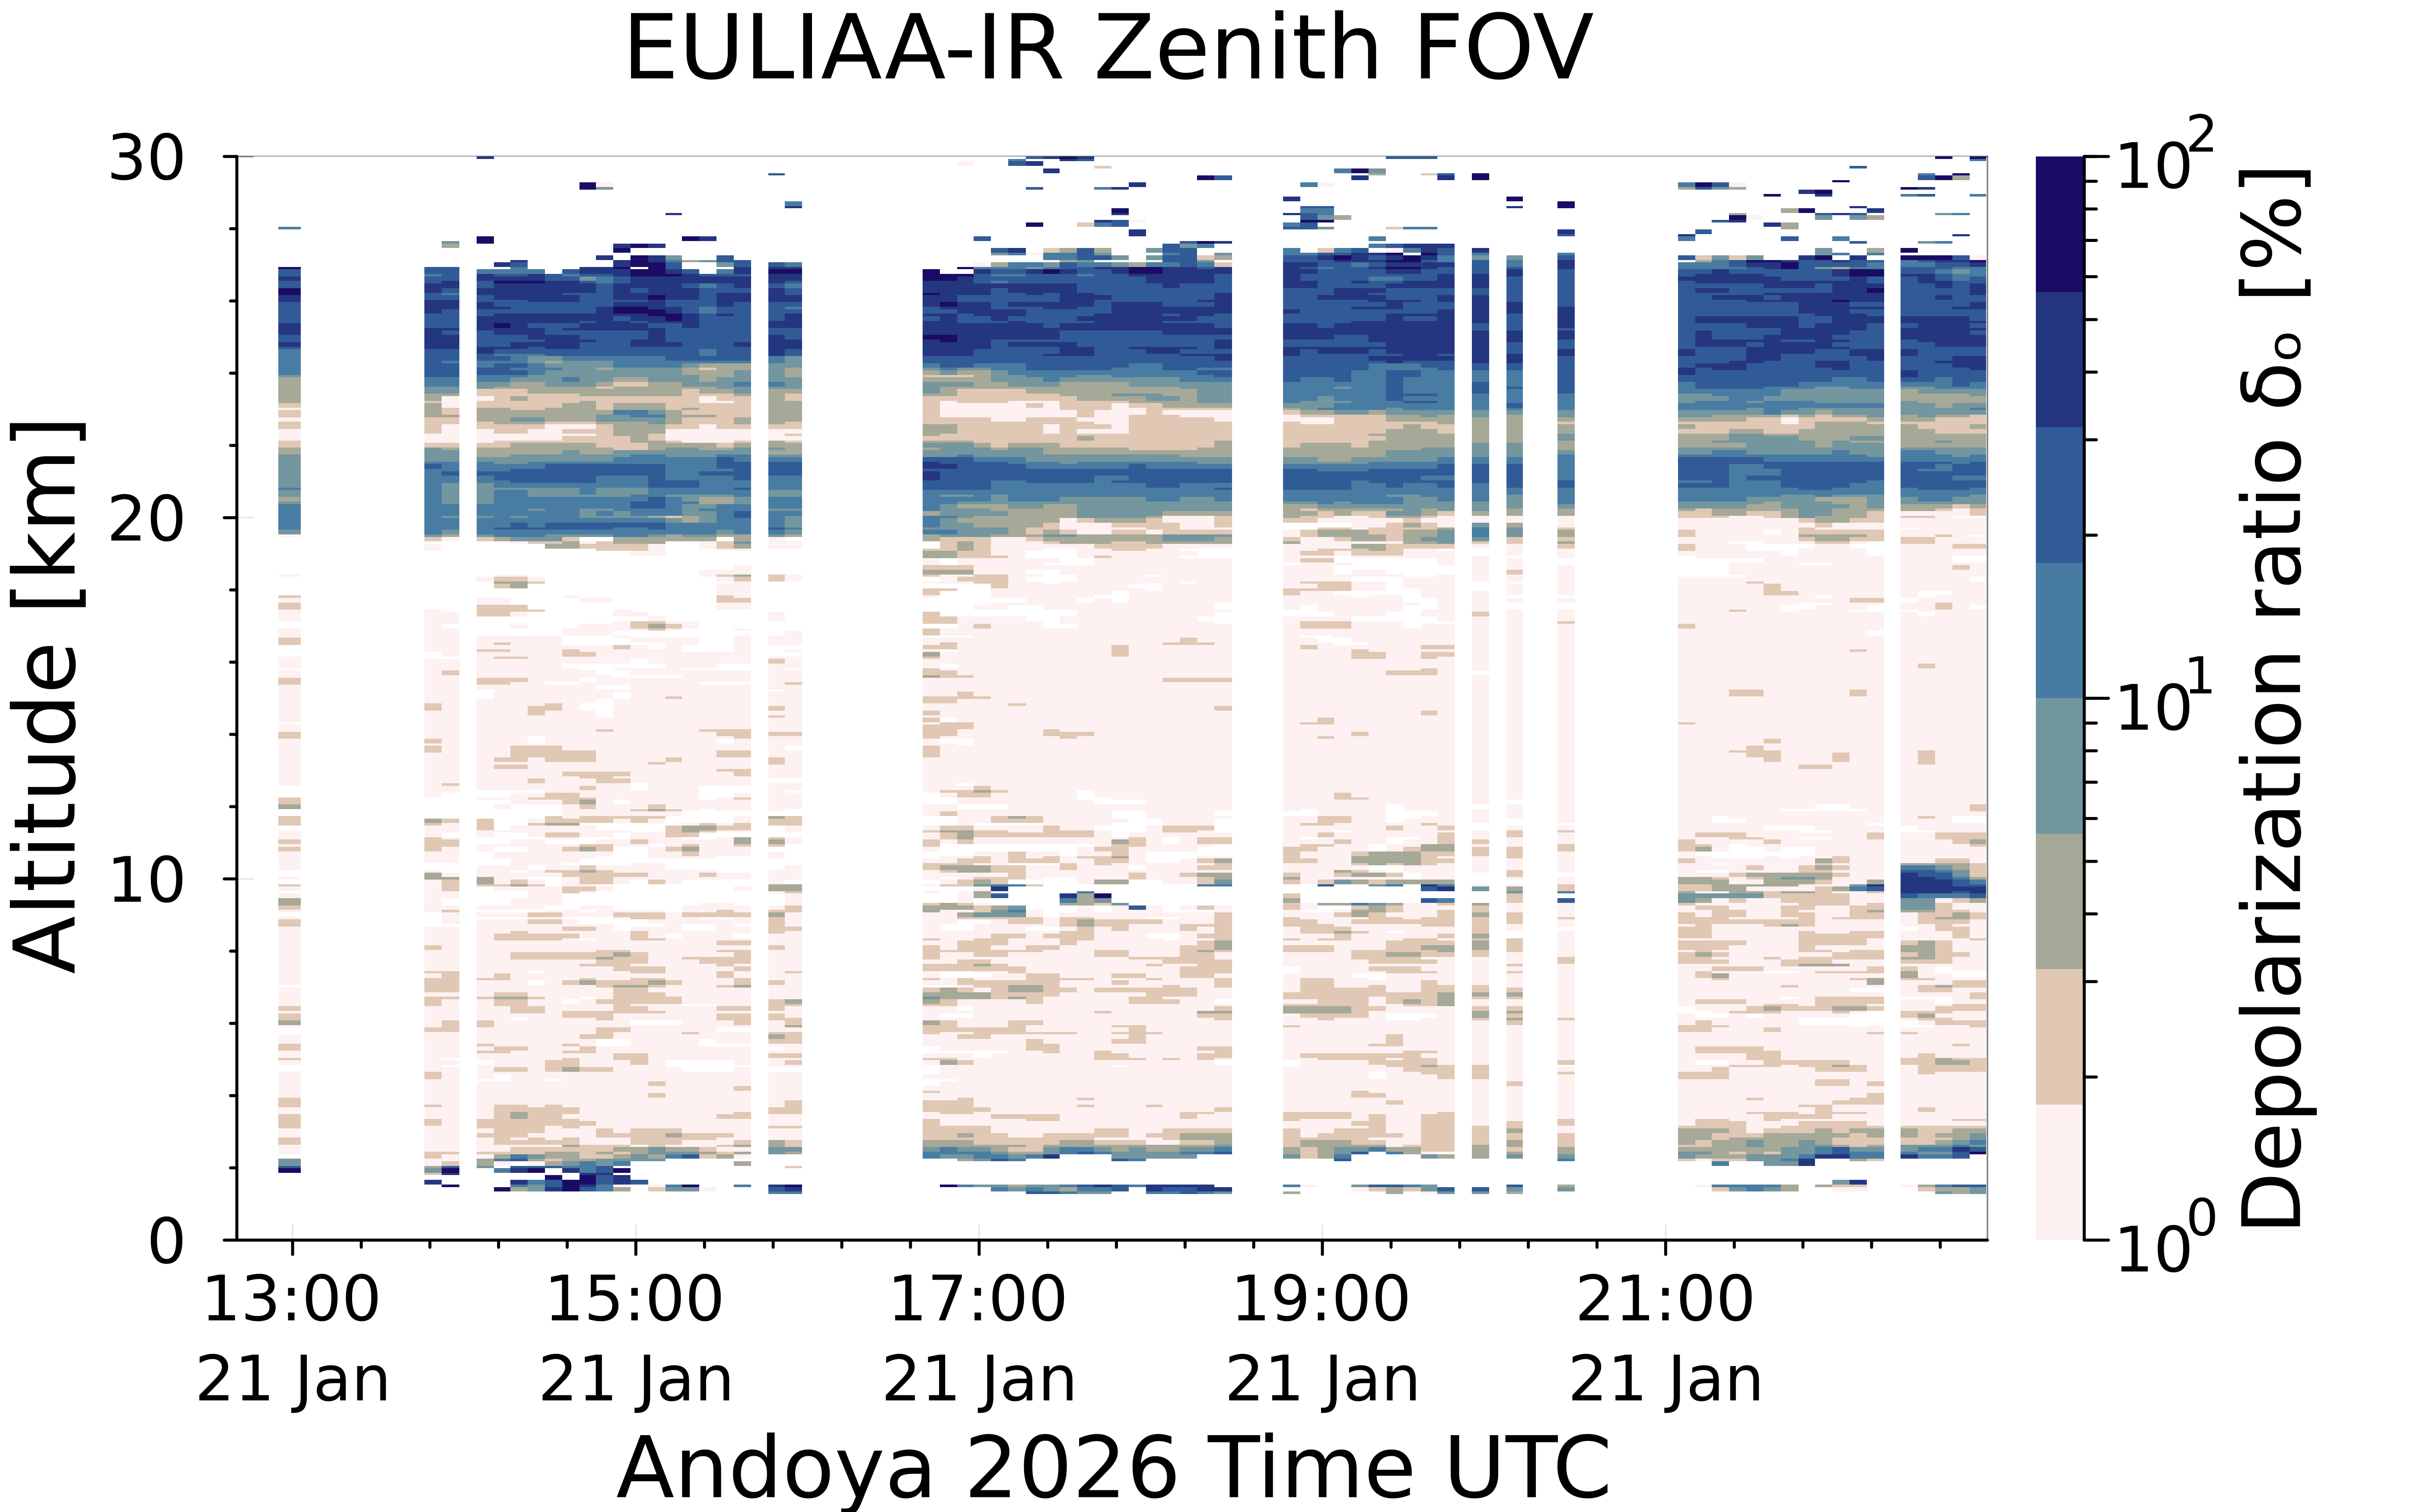
\includegraphics[width=.20\linewidth]{EULIAA_L1_2026-01-21_12-48-00_dT15min_dH200m_OL_DEPOL_ZFOV_13_00_21_00.png} &
		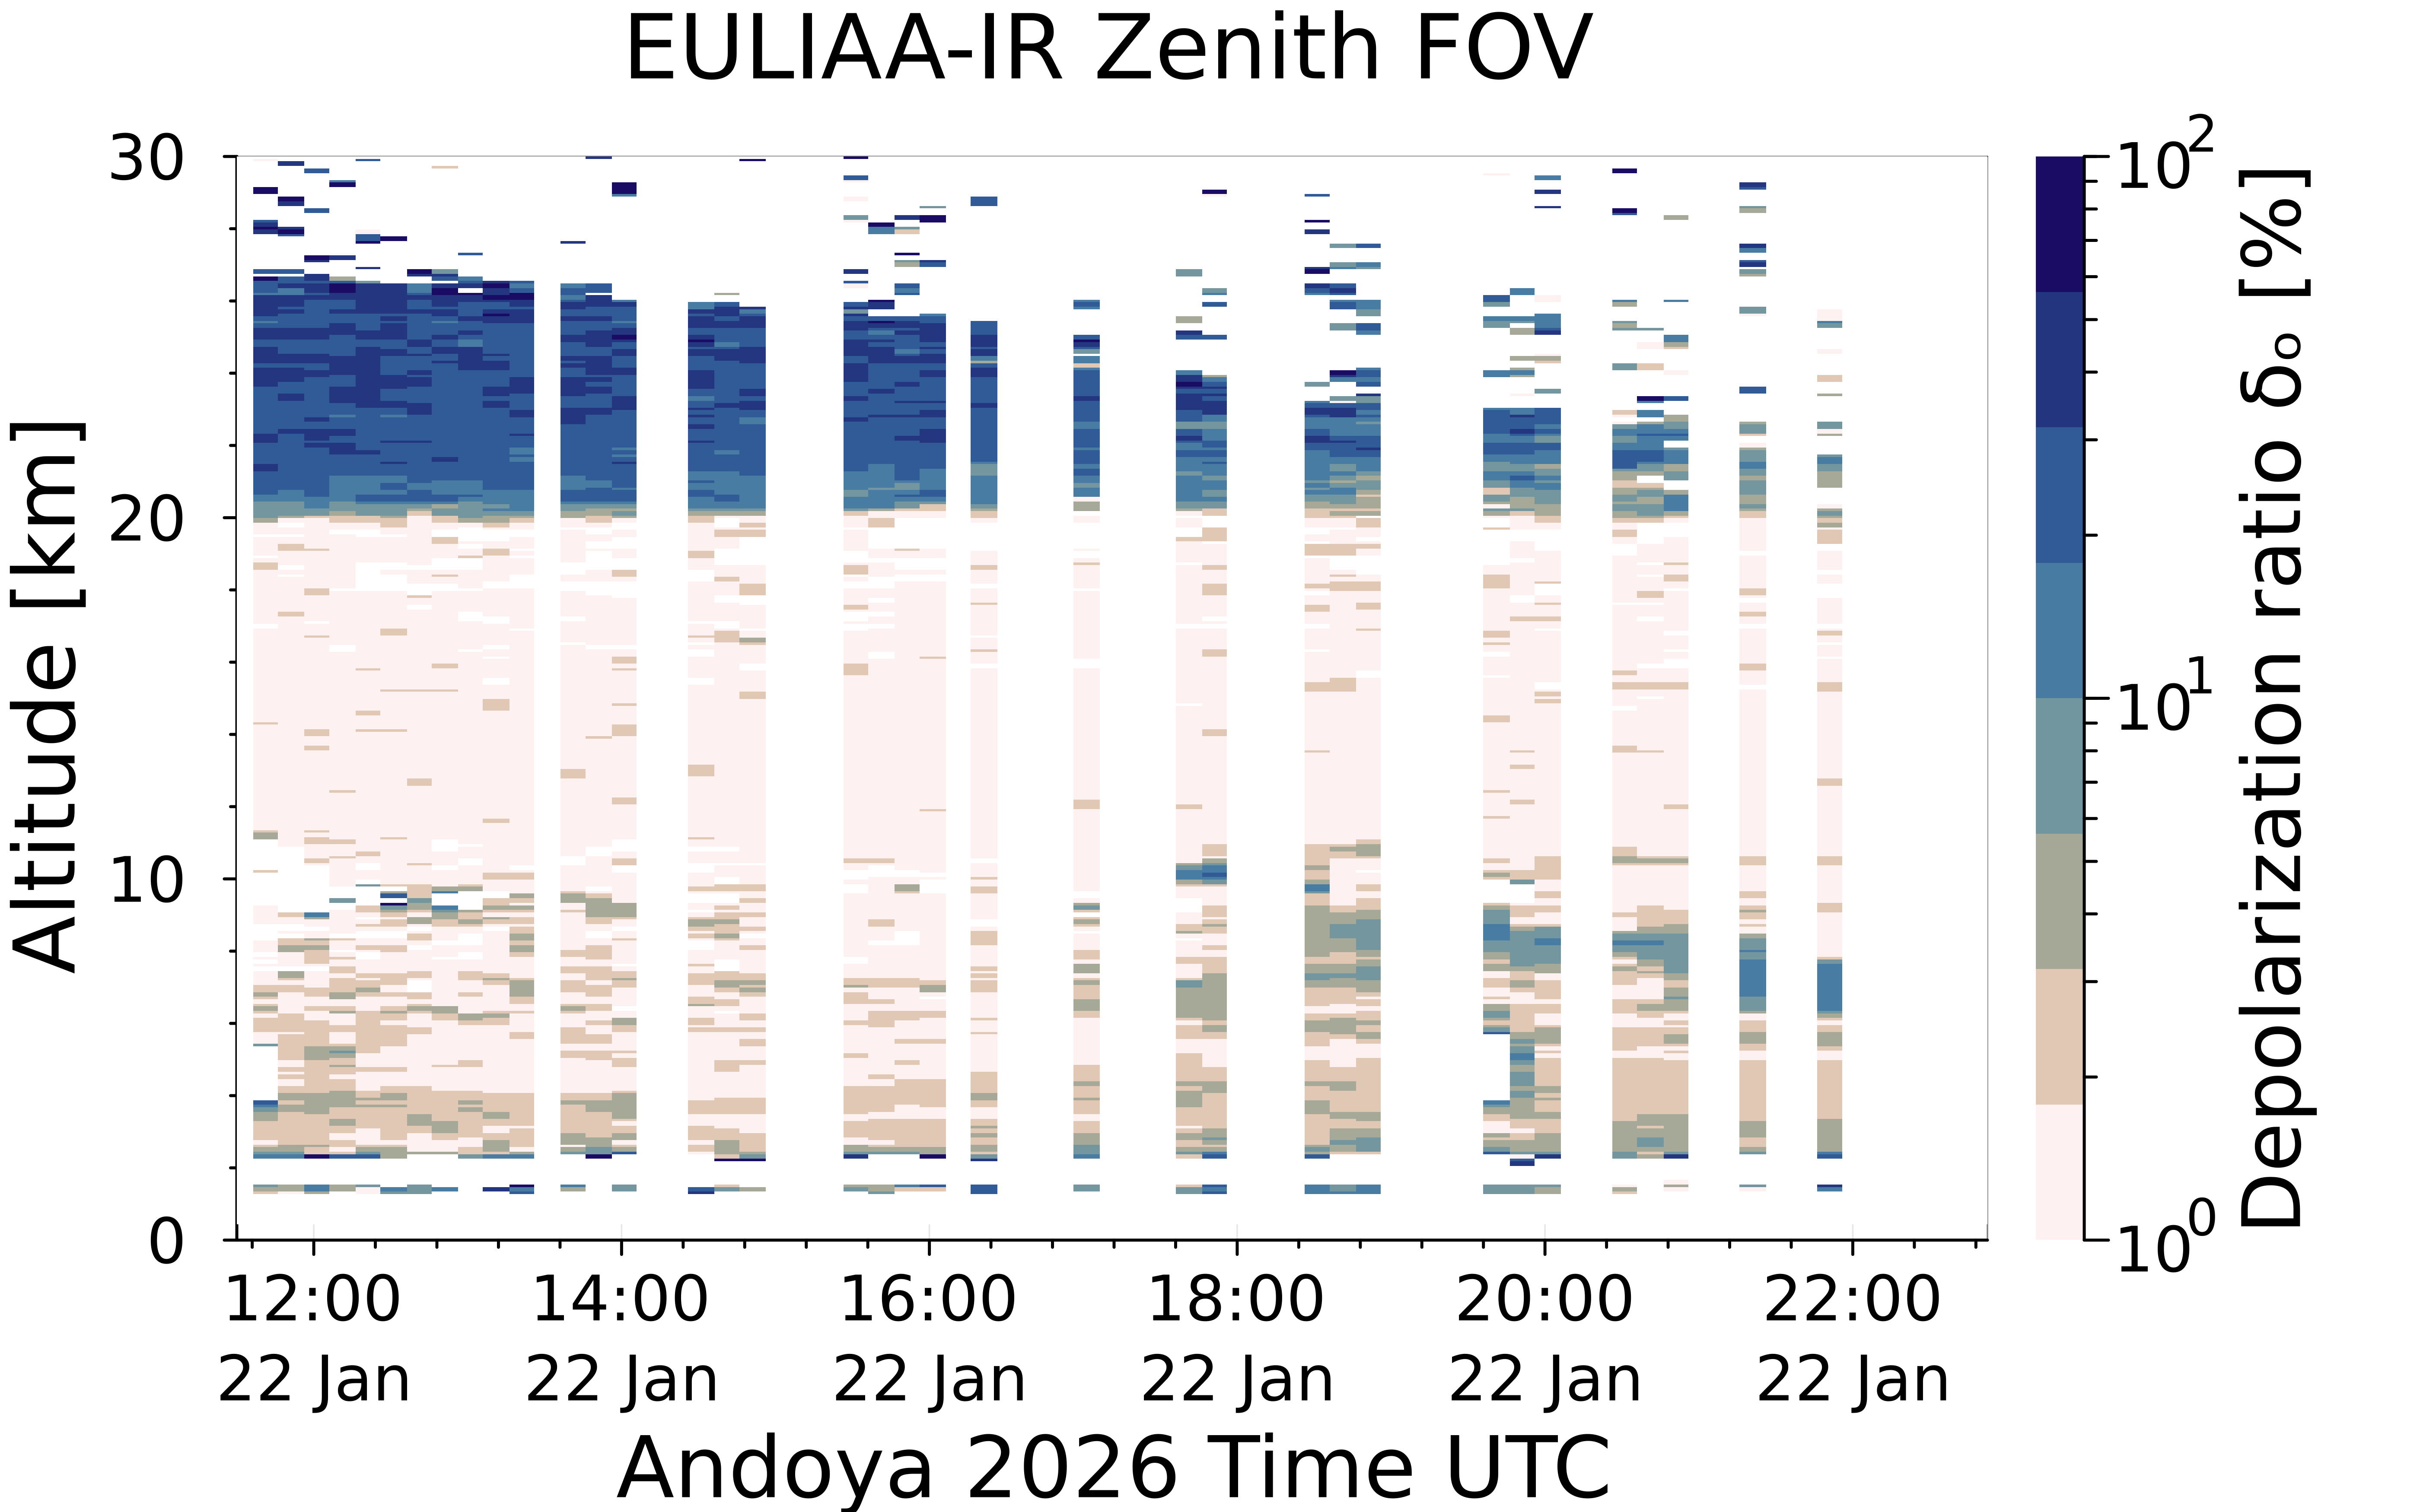
\includegraphics[width=.20\linewidth]{EULIAA_L1_2026-01-22_00-00-00_dT15min_dH200m_OL_DEPOL_ZFOV_12_00_22_00.png} &
		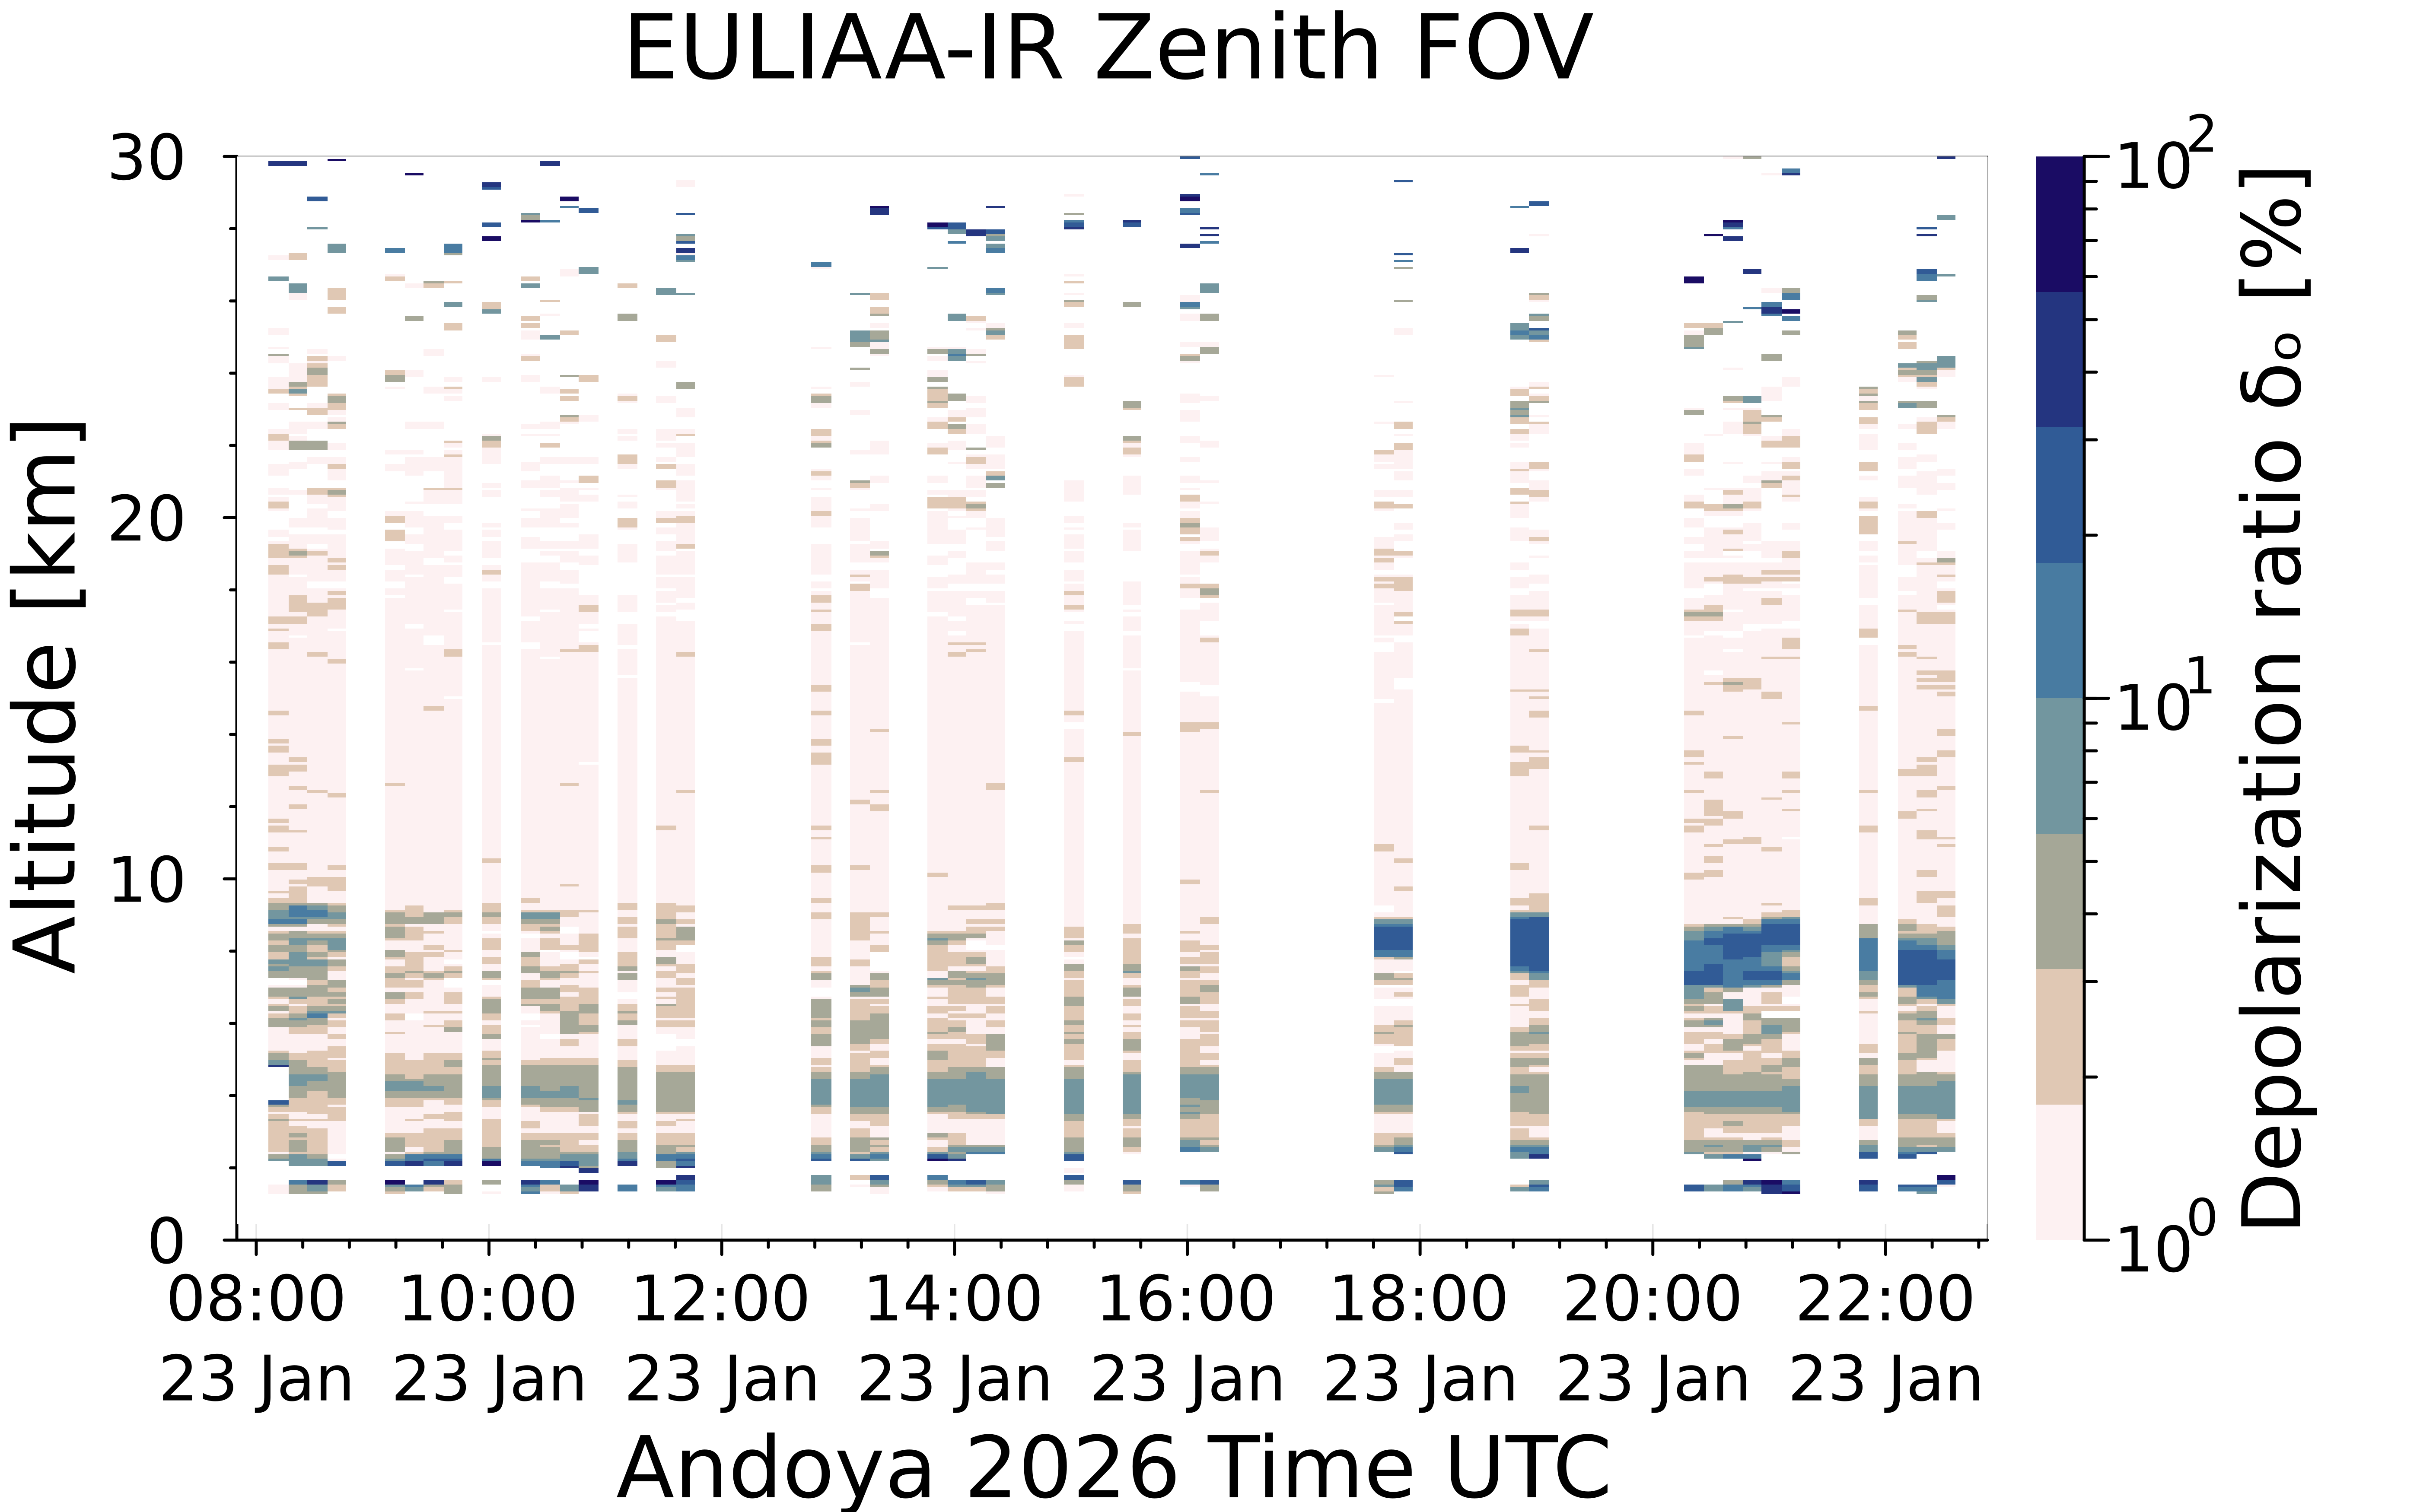
\includegraphics[width=.20\linewidth]{EULIAA_L1_2026-01-23_00-00-00_dT15min_dH200m_OL_DEPOL_ZFOV_08_00_22_00.png} &
		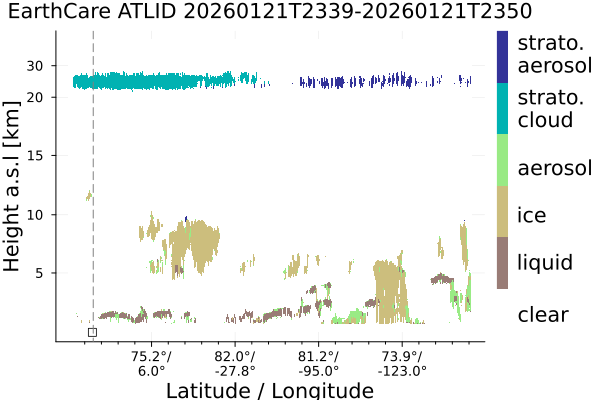
\includegraphics[width=.20\linewidth]{EarthCare_ATLID_20260121T2339-20260121T2350_classific.png}
		\\
		
		% Row with classification:
		\multicolumn{4}{l}{\vspace{+1em}\colouredcircle {\large Towards a aerosol/PSC classification based temperature clustering in the $\beta_p$~-~$\delta_\circ$ space is shown below $\downarrow$.\hfill}} &\\
		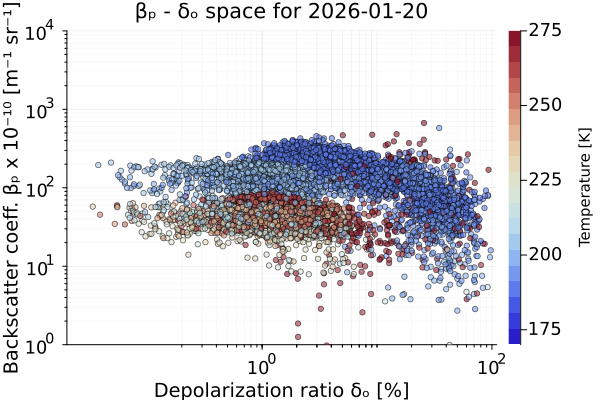
\includegraphics[width=.20\linewidth]{EULIAA_L1_2026-01-20_16-36-00_dT15min_dH200m_OL_DEBSC_ZFOV_17_00_20_00.png} &
		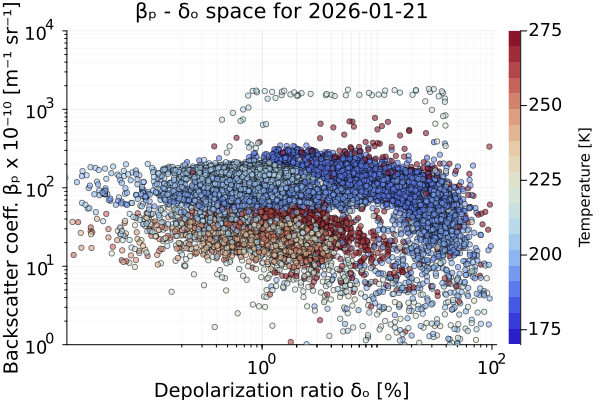
\includegraphics[width=.20\linewidth]{EULIAA_L1_2026-01-21_12-48-00_dT15min_dH200m_OL_DEBSC_ZFOV_13_00_21_00.png} &
		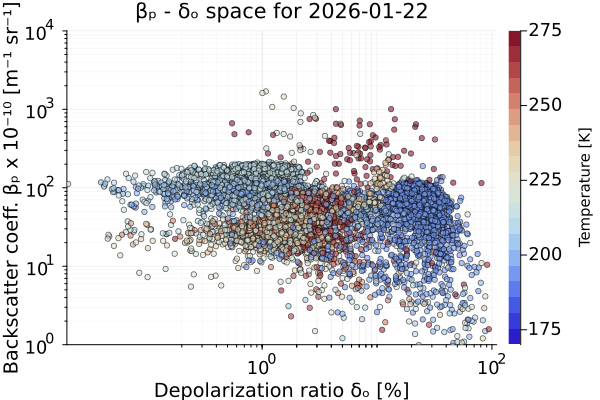
\includegraphics[width=.20\linewidth]{EULIAA_L1_2026-01-22_00-00-00_dT15min_dH200m_OL_DEBSC_ZFOV_12_00_22_00.png} &
		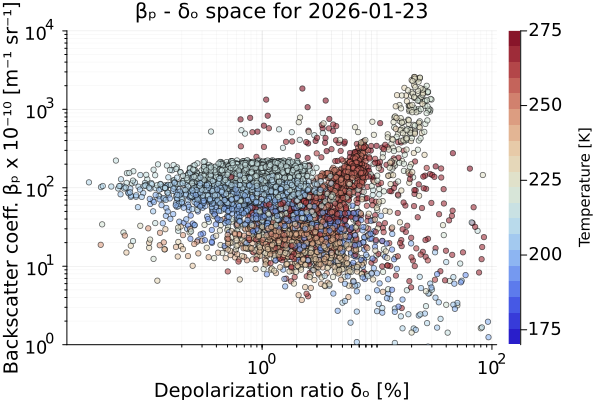
\includegraphics[width=.20\linewidth]{EULIAA_L1_2026-01-23_00-00-00_dT15min_dH200m_OL_DEBSC_ZFOV_08_00_22_00.png} & 
		\begin{minipage}{0.18\linewidth}
			\vspace{-20em}
			{\large $\uparrow$ EarthCARE ATLID lidar confirmed the presence of PSC and stratospheric aerosol on 21st Jan 2026.
			Top: particle backscatter  $\beta_p$\@~355~nm. Middle: depolarization ratio. Bottom: target classification. The black square at $\approx$380~m indicates the location of \euliaa lidar.}	
		\end{minipage}
		\\
	\end{tabular}
\end{minipage}

%\multicolumn{4}{l}{\vspace{+1em}\colouredcircle {\large The EarthCARE \hfill}} & \\
%	\begin{minipage}{0.15\linewidth}
%		\begin{center}
			%\setcaptiontype{figure}
%			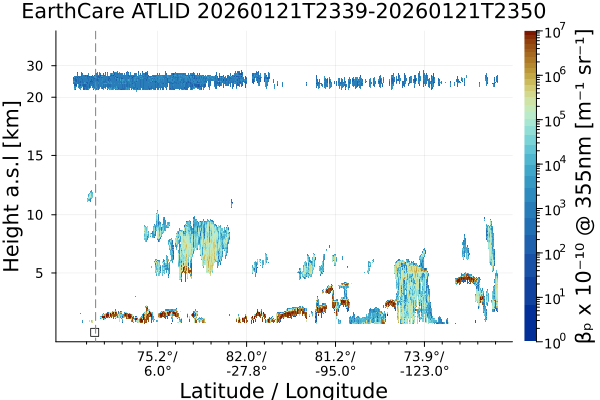
\includegraphics[width=.75\linewidth]{EarthCare_ATLID_20260121T2339-20260121T2350_backsct.png}\\
%			\captionsetup{width=0.8\linewidth}
%			\captionof{figure}{EarthCARE $\beta_p$.}
%			\label{fig:ec_beta}
%		\end{center}
%	\end{minipage}
%	&
%	\begin{minipage}{0.25\linewidth}	
%		\begin{center}             
			%\setcaptiontype{figure}
%			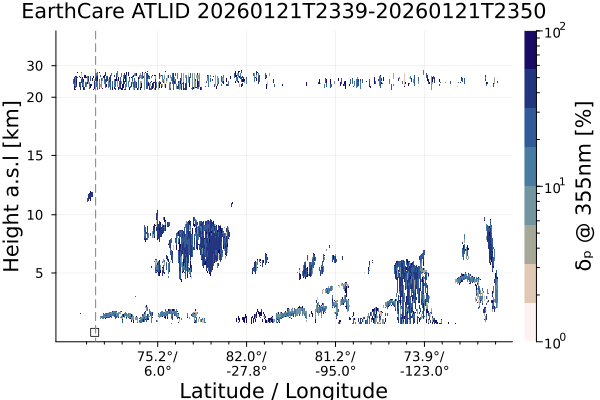
\includegraphics[width=.75\linewidth]{EarthCare_ATLID_20260121T2339-20260121T2350_depol.png}\\
%			\captionsetup{width=0.9\linewidth}
%			\captionof{figure}{EarthCARE depolarization.}
%			\label{fig:ec_depol}
%		\end{center}
%	\end{minipage}
%	&
%	\begin{minipage}{0.25\linewidth}	
%		\begin{center}             
			%\setcaptiontype{figure}
%			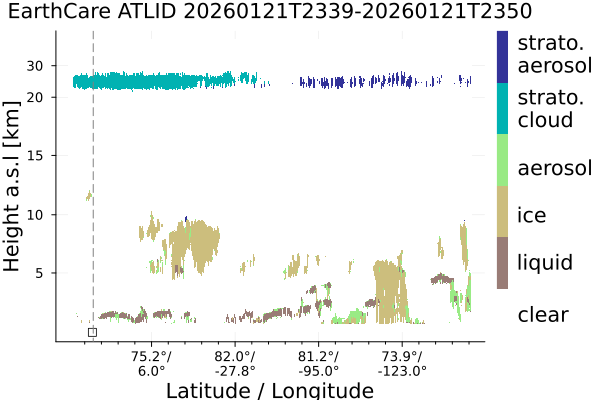
\includegraphics[width=.75\linewidth]{EarthCare_ATLID_20260121T2339-20260121T2350_classific.png}\\
%			\captionsetup{width=0.9\linewidth}
%			\captionof{figure}{EarthCARE target classification.}
%			\label{fig:ec_classfic}
%		\end{center}
%	\end{minipage}
%	 &
	
	%\multicolumn{2}{l}{\vspace{+5em}
	

 %(with $\Delta T=T_{top}-T_{base}$ and $\Delta H=CTH-CBH$ .
 
   
%\parbox[l]{0.8\linewidth}{   \vspace{-.5em}
%	{Some text here....}    
%}
}

%%%%%%%%%%%%%%%%%%%%%%%%%%%%%%%%%%%%%%%%%%%%%%%%%%%%%%%%%%%%%%%%%%%%%%%%%%%%%%
\headerbox{4.- Conclusions}{name=conclutions,column=1,span=1,below=results}{
  %%%%%%%%%%%%%%%%%%%%%%%%%%%%%%%%%%%%%%%%%%%%%%%%%%%%%%%%%%%%%%%%%%%%%%%%%%%%%%
{\normalsize
\begin{itemize}
		\item First mobile \euliaa lidar observations has demonstrated its unique capabilities as no other mobile system,
		\item Aerosols in the stratosphere can be observed even under the presence of thin clouds,
		\item The circular polarization the system uses needs to be further studied since most of studies use linear polarization,
\end{itemize}
}
% \sc (this make cool big font)!
}

%%%%%%%%%%%%%%%%%%%%%%%%%%%%%%%%%%%%%%%%%%%%%%%%%%%%%%%%%%%%%%%%%%%%%%%%%%%%%%
\headerbox{5.- References }{name=references,column=2, span=2, below=results}{
%%%%%%%%%%%%%%%%%%%%%%%%%%%%%%%%%%%%%%%%%%%%%%%%%%%%%%%%%%%%%%%%%%%%%%%%%%%%%%
%\colouredcircle \hspace{2em}
\hspace{-2.4em}
\begin{minipage}{0.99\linewidth}
{\small
	\begin{enumerate}
		\setlength\itemsep{0.08em}
		\item J. Höffner, J. Froh, T. H. Mense, A. Munk, G. Baumgarten, M. Strotkamp, “General purpose Doppler LiDAR for validation and space”, Proc. SPIE ICSO, (2025): https://doi.org/10.1117/12.3072762
		\item J. Höffner, J. Froh, T. Mense, A. Mauer, M. Strotkamp, A. Munk, B. Jungbluth, H.-D. Hoffmann, “Ground-based general purpose Doppler-lidar: a technology for Doppler-aerosol measurements and beyond”, in Proc. SPIE (2020): https://doi.org/10.1117/12.2599364
		\item Lübken, Franz-Josef, and Josef Höffner. “VAHCOLI, a New Concept for Lidars: Technical Setup, Science Applications, and First Measurements”. AMT (2021): https://doi.org/10.5194/amt-14-3815-2021.
		\item EULIAA website: \url{https://euliaa.eu}
	\end{enumerate}
}	
\vspace{-0.6em}
\end{minipage}
	%\end{tabular}
	%\vspace{0.5em}
}
%%%%%%%%%%%%%%%%%%%%%%%%%%%%%%%%%%%%%%%%%%%%%%%%%%%%%%%%%%%%%%%%%%%%%%%%%%%%%%
\headerbox{Acknowledgements}{name=acknown,column=0, span=1, below=andoya}{
	%%%%%%%%%%%%%%%%%%%%%%%%%%%%%%%%%%%%%%%%%%%%%%%%%%%%%%%%%%%%%%%%%%%%%%%%%%%%%%
	{This research is founded under EULIAA: Project-ID: 101086317. Authors thank to the Alomar technical staff for supporting measurements.
	}\\
	\hfill
\includegraphics[width=0.35\linewidth]{FundedbytheEU.png}
}
%%%%%%%%%%%%%%%%%%%%%%%%%%%%%%%%%%%%%%%%%%%%%%%%%%%%%%%%%%%%%%%%%%%%%%%%%%%%%%%%%%
%\headerbox{[*] Contact}{name=contact, column=2, below=results}{
%{\Large \color{white}{Email:	pablo.saavedra@uni-leipzig.de}}\\
%\hspace{3em}\includegraphics[scale=0.04]{github_pablosaa.png}\hspace{3em}
%\includegraphics[scale=0.16]{twitter_DunkleWolke.png}
%}

\end{poster}

\end{document}

%%%%%%%%%%%%%%%%%%%%%%%%%%%%%%%%%%%%%%%%%%%%%%%%%%%%%%%%%%%%%%%%%%%%%%%%%%%%%%%
